%!TeX spellcheck = fr_FR
\documentclass[letterpaper, 12pt]{article}
\usepackage[top = 1.6cm, left = 2cm, right = 2cm ]{geometry}
\usepackage[pdftex]{graphicx}
\usepackage{soulutf8}
\usepackage{amsmath}
\usepackage{tikz}
\usepackage[colorlinks=true, urlcolor=blue, linkcolor=darkgray, citecolor=darkgray]{hyperref}
\usepackage[utf8]{inputenc}
\usepackage{longtable}
\usepackage[T1]{fontenc}
\usepackage{epigraph}
\usepackage{fancyhdr}
\usepackage{float}
\usepackage{subfig}
\usepackage{xcolor}
\usepackage{eurosym}
\usepackage{calc}
\usepackage{multirow} 
%
%
%%%%% Custom commands
%
%
\def\changemargin#1#2{\list{}{\rightmargin#2\leftmargin#1}\item[]}
\let\endchangemargin=\endlist 
%
\newcommand{\newlinealinea}{
~\\ \hspace*{0.5cm}}
%
\newcommand{\alinea}{
\hspace*{0.5cm}}
%
\newcommand{\alinealong}{
\hspace*{1.1cm}}
%
\newcommand{\alignparagraph}{
\hspace*{0.6cm}}
%
\newcommand{\red}[1]{
	\textcolor{red}{#1}}
%
\newcommand{\green}[1]{
	\textcolor{green}{#1}}
%
\newcommand{\point}{$\bullet\ $}
%
\makeatletter
	\newcommand*{\whiten}[1]{\llap{\textcolor{white}{{\the\SOUL@token}}\hspace{#1pt}}}
	\newcommand{\myul}[1]{
		\underline{\smash{#1}}
	}
\makeatother
%
\setlength{\fboxsep}{2pt}
%
\DeclareMathOperator*{\argmax}{\arg\!\max}
%
%
%%%%% Custom text
%
%
\makeatletter
\@addtoreset{section}{part}
\makeatother  
\renewcommand\partname{Partie} 
%
\renewcommand*\sfdefault{phv}
\renewcommand*\rmdefault{ppl}
%
\renewcommand\epigraphflush{flushright}
\renewcommand\epigraphsize{\normalsize}
\setlength\epigraphwidth{0.7\textwidth}
%
\definecolor{titlepagecolor}{cmyk}{0.24,0.92,0.78,0.25}
\definecolor{red}{cmyk}{0, 0.91, 0.91, 0.20}
%
\DeclareFixedFont{\titlefont}{T1}{phv}{\seriesdefault}{n}{0.375in}
%
%
%%%%% Header
%
%
\pagestyle{fancy}
\lhead{Anthony Rouneau}
\rhead{MAB2 Sciences Informatiques}
\cfoot{\thepage}
%
%
%%%%% Title page. The following code is borrowed from: 
%%%%%       http://tex.stackexchange.com/a/86310/10898
%
%
\newcommand\titlepagedecoration{%
\begin{tikzpicture}[remember picture,overlay,shorten >= -10pt]

\coordinate (aux1) at ([yshift=-70pt]current page.north east);
\coordinate (aux2) at ([yshift=-460pt]current page.north east);
\coordinate (aux3) at ([xshift=-6cm]current page.north east);
\coordinate (aux4) at ([yshift=-150pt]current page.north east);

\begin{scope}[titlepagecolor!40,line width=12pt,rounded corners=12pt]
\draw
  (aux1) -- coordinate (a)
  ++(225:5) --
  ++(-45:5.1) coordinate (b);
\draw[shorten <= -10pt]
  (aux3) --
  (a) --
  (aux1);
\draw[opacity=0.6,titlepagecolor,shorten <= -10pt]
  (b) --
  ++(225:2.2) --
  ++(-45:2.2);
\end{scope}
\draw[titlepagecolor,line width=8pt,rounded corners=8pt,shorten <= -10pt]
  (aux4) --
  ++(225:0.8) --
  ++(-45:0.8);
\begin{scope}[titlepagecolor!70,line width=6pt,rounded corners=8pt]
\draw[shorten <= -10pt]
  (aux2) --
  ++(225:3) coordinate[pos=0.45] (c) --
  ++(-45:3.1);
\draw
  (aux2) --
  (c) --
  ++(135:2.5) --
  ++(45:2.5) --
  ++(-45:2.5) coordinate[pos=0.3] (d);   
\draw 
  (d) -- +(45:1);
\end{scope}
\end{tikzpicture}%
}
%
\begin{document}
	\begin{titlepage}
	%
	\noindent
	%
	\newgeometry{bottom = 2cm, top = 2.5cm}
	\begin{center}
		
\includegraphics[scale=1.2]{Images/UMONS}\\
			\vspace*{0.3cm}
		
\includegraphics[scale=0.23]{Images/FS_Logo}\\
			\vspace*{2.5cm}
		%
		\titlefont Audio Processing\\~\\ {\huge Résumé} \par
		%
	\end{center}
	\vspace*{3cm}
	\hfill
	%
	\begin{minipage}{0.04\linewidth}
		\begin{flushright}
			\rule{0.5pt}{100pt}
		\end{flushright}
	\end{minipage}
	%
	\begin{minipage}{0.95\linewidth}
		\begin{flushleft}
			\textsf{\textbf{Résumé réalisé par :}} Anthony Rouneau\\
			\textsf{\textbf{Aidé par :}} Maximilien Charlier\\
			\textsf{\textbf{Section :}} 2$^{\text{\`eme}}$ Bloc Master en 
				Sciences Informatiques\\
			\textsf{\textbf{Images :}} Proviennent du cours de M. Dutoit, M. Dupont et M. D'Alessandro.\\
		\end{flushleft}
	\end{minipage}
	%
	\vspace*{\fill}                                                             
	%
	\begin{center}
		Faculté des Sciences $\bullet$ Université de Mons $\bullet$ 
		Place du Parc 20 $\bullet$ B-7000 Mons
	\end{center}
	%
	\titlepagedecoration
	%
\end{titlepage}
%
%
%%%% Tables des matières
%
%
\newgeometry{top = 3cm, left = 2cm, right = 2cm, bottom=2.5cm}
%
\tableofcontents
%
\newpage
%
%
\part{Dutoit -- Analyse bas niveau}
	\section{Cell phone}
		\subsection{Analyse du fichier audio}
			\subsubsection*{Spectrogramme}
				\alinea On utilise une \hl{fenêtre de pondération} pour afficher un spectrogramme. Au plus la taille de cette fenêtre 
					est élevée, au plus on a de détails. Inversement, si on prend une petite fenêtre, on aura une vision globale, plus 
					générale. \hl{Les différentes tailles ont chacune leurs avantages et inconvénients}. Un spectrogramme met en évidence
					les \hl{formants}, qui peuvent être lu et reconnus par des spécialistes. Les fréquences sont sur l'axe vertical,
					le temps sur l'axe horizontal, et l'intensité en couleur. Exemple de spectrogramme détaillé (plus précis sur les
					couleurs) :
				%
				\begin{center}
					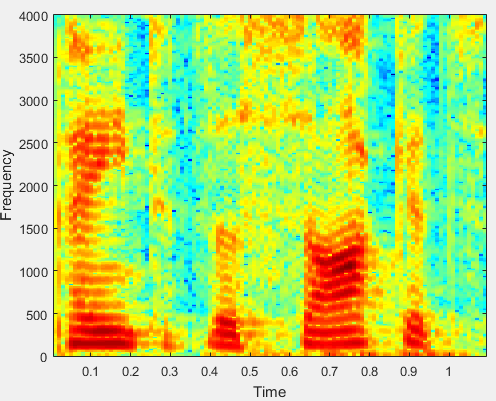
\includegraphics[width=3in]{Images/spectrogram}
				\end{center}
				%
				On affiche souvent un spectrogramme sur le fichier audio complet, ou en tout cas sur plusieurs mots.
				%
			%
			\subsubsection*{Périodogramme}
				\alinea Donne la \red{densité spectrale de puissance}.
					L'axe horizontal affiche les fréquences (souvent normalisée pour représenter les fréquences entre 0 et Fe/2),
					tandis que l'axe vertical donne l'amplitude. Le périodogramme s'applique généralement sur une lettre (voyelle) afin
					d'en identifier les formants. Dans l'exemple suivant, Fe = 8kHz. On a donc 1 = 4kHz. On identifie
					la \hl{fondamentale} à 125Hz (premier pic), et ses \hl{formants} (pics de plus haute amplitude) en 300,
					1400 et 2700Hz.
				%
				\begin{center}
					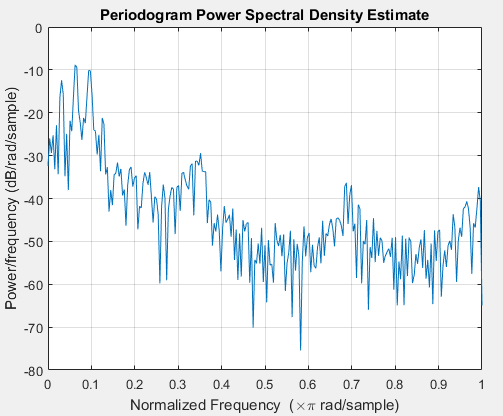
\includegraphics[width=3in]{Images/periodogram}
				\end{center}
				%
			%
		%
		\subsection{Prédiction linéaire (LP) sur un segment}
			\subsubsection*{Coarticulation}
				\alinea La \red{coarticulation} est un problème venant du fait que la \hl{prononciation d'un son} dépend du son qui 
					le précède et du son qui le suit. \c Ca vient du fait que les cordes vocales sont "mécaniques" et présentent 
					une inertie.
				%
			%
			\subsubsection*{Son voisé ($\sim$voyelle)}
				\alinea On va chercher 10 coefficients ($A_z$) qui représente les positions de formants dans la parole. On va ensuite
					pouvoir retrouver cette voix (la générer) grâce à un filtre tous-pôles ($\frac{1}{A_z}$)\footnote{\texttt{freqz} permet
					d'obtenir la réponse en fréquence d'un filtre et son amplitude à partir de coefficients $A_z$}. 
					Si on passe le signal de base par le filtre\footnote{\texttt{filter} permet d'appliquer un filtre à des échantillons.}
					inverse de génération ($A_z$, qui est l'inverse de $\frac{1}{A_z}$), on obtient le \red{résidu du signal}, c'est à dire 
					l'\hl{excitation sonore} (indépendante de la lettre formée) qui va définir la \hl{position des harmoniques et le pitch 
					du son}.
				%
			\subsubsection*{Son non-voisé ($\sim$consonne)}	
				\alinea Dans ce cas-ci, on va préférer utiliser un périodogramme moyenné (\texttt{pwelch}) afin d'avoir une 
					meilleure estimée de la densité spectrale de puissance. L'excitation peut être générée à partir de 
					données aléatoires (bruit blanc).
				%		
			%
		%
		\subsection{Prédiction linéaire sur le son entier (5400bits/s)}
			\subsubsection*{Pitch constant}
				\alinea Le truc ici est de générer une excitation qui restera la même pour tout segment de \hl{10ms de voix}.
					On obtient alors un son très métallique, très peu naturel. Pour bien faire, on doit prendre en 
					compte l'itération d'avant (retard $z$) dans le filtrage afin que toutes les frames soient correctement liées.
					De plus, on doit faire attention à ce que les excitations (impulsions de Dirac) 
					se rejoignent correctement (décalage nécessaire dans le cas
					ou le nombre de segment choisi n'est pas un multiple de la fréquence d'échantillonnage).
				%
			%
			\subsubsection*{Pitch adaptatif}
				\alinea Pour chaque frame, on va analyser le pitch et générer une excitation qui y correspondra. On doit faire
					attention au décalage qui est nécessaire pour lier les différentes excitation tout en gardant des fenêtres de 
					$10ms$.
				%
			%
			\subsubsection*{LPC10 (2400bits/s)}
				\alinea Le même principe, mais avec des fenêtres plus grandes : $22.5ms$.
			%
		%
		\subsection{CELP (14kbits/s)}
			\alinea Le principe ici est de générer aléatoirement un \hl{dictionnaire d'excitations}, que l'on va \hl{filtrer par les
				coefficients de l'analyse LPC} afin d'avoir des excitations plus riches que de simples impulsions de Dirac.
			%
		%
	%
	\section{MP3}
		\subsection{Principe général}
			\alinea Le principe général de la compression MP3 est d'ajuster la quantization du son en fonction de ce qui est 
				audible ou pas. En effet, on peut\hl{ augmenter le ratio signal sur bruit} (S/N) en \hl{augmentant le bit rate},
				mais ce n'est pas nécessaire de le faire sur toutes les bandes de fréquence de la même fa\c con. C'est pourquoi
				on va utiliser un modèle de perception qui va nous guider pour savoir quelles bandes de fréquence améliorer et
				quelles bandes de fréquence il faut 'laisser à l'abandon'.
			%
		%
		\subsection{Analyse d'erreur par bande de fréquence}
			\alinea Pour réaliser la compression, on a besoin d'ajuster chaque bande de fréquence. C'est pourquoi on aura également
				besoin de sous-échantillonner les signaux pour pouvoir reconstruire le signal final. En effet, si on divise le
				signal original en $M$ bandes de fréquences, on aura $M$ fois plus d'échantillons que le signal original. Ensuite,
				on peut le passer dans un filtre "escalier" afin de le digitaliser. Si l'on veut retrouver le même nombre 
				d'échantillons qu'avant le scaling, on va devoir sur-échantillonner. C'est ce qu'on appelle le sub-band filtering.
				Le principe est donc de \hl{retirer des échantillons, de les remplacer par des zeros, et ensuite de passer le tout dans un
				filtre qui va donner de la "couleur" à ces zéros}.
			%
			\begin{center}
				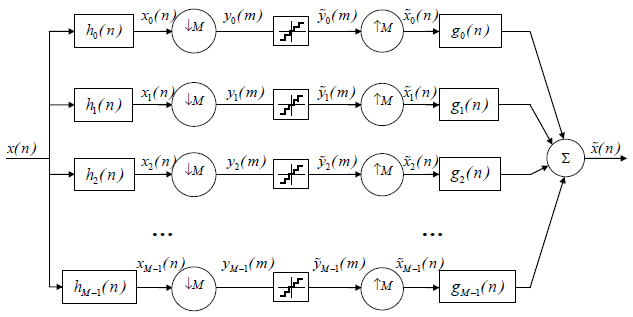
\includegraphics[width=4in]{Images/subband} \hfill 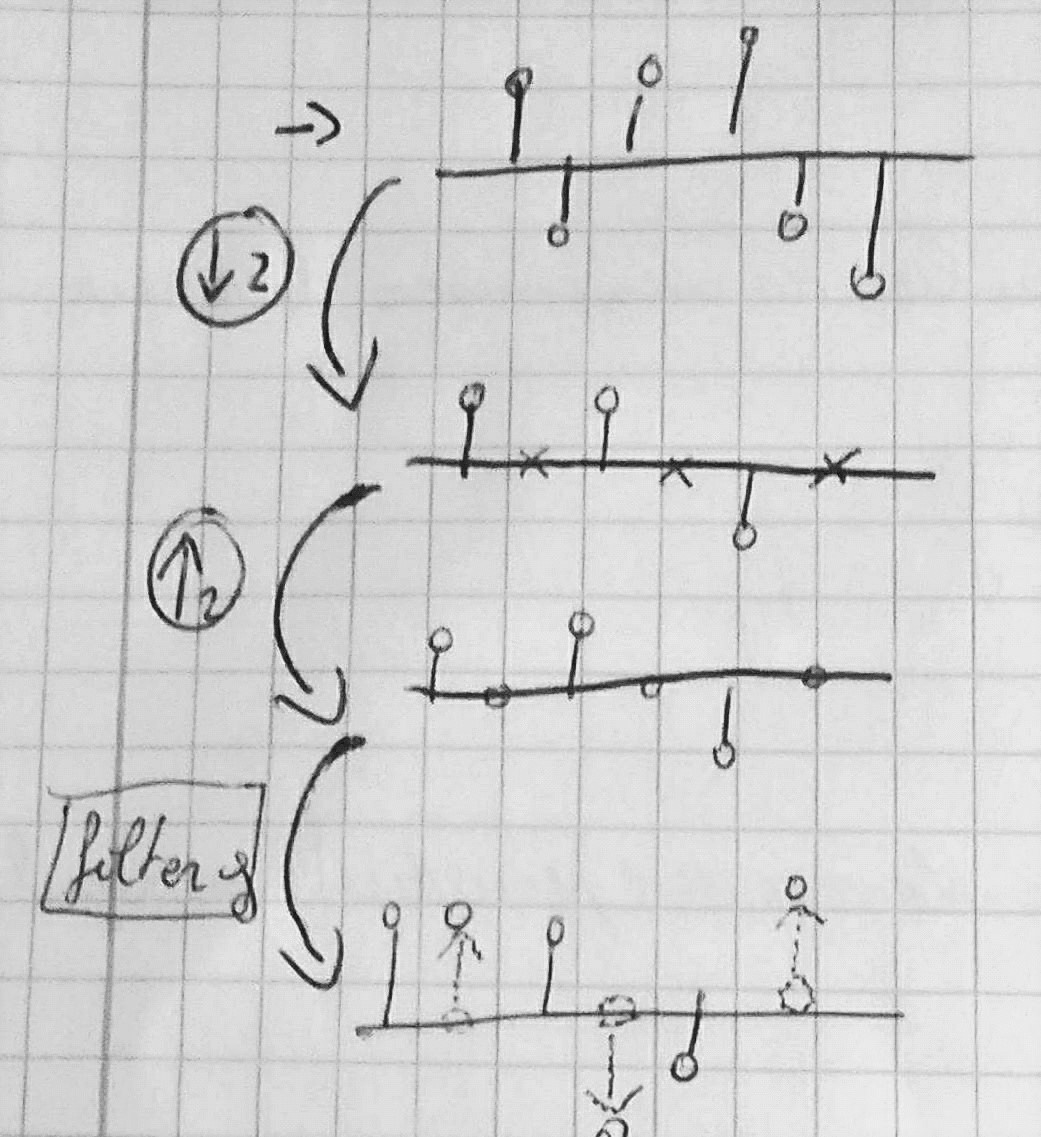
\includegraphics[width=2in]{Images/subband2}
			\end{center}
			%
			\alinea En prenant un exemple, si on effectue cette opération sur un 'chirp', on aura un recouvrement total du spectre.
				En effet, les filtres utilisés avant et après la digitalisation ne sont pas "idéaux", et ajoutent de l'erreur.
				On a alors un effet de 'miroir en quadrature' :
				\begin{center}
					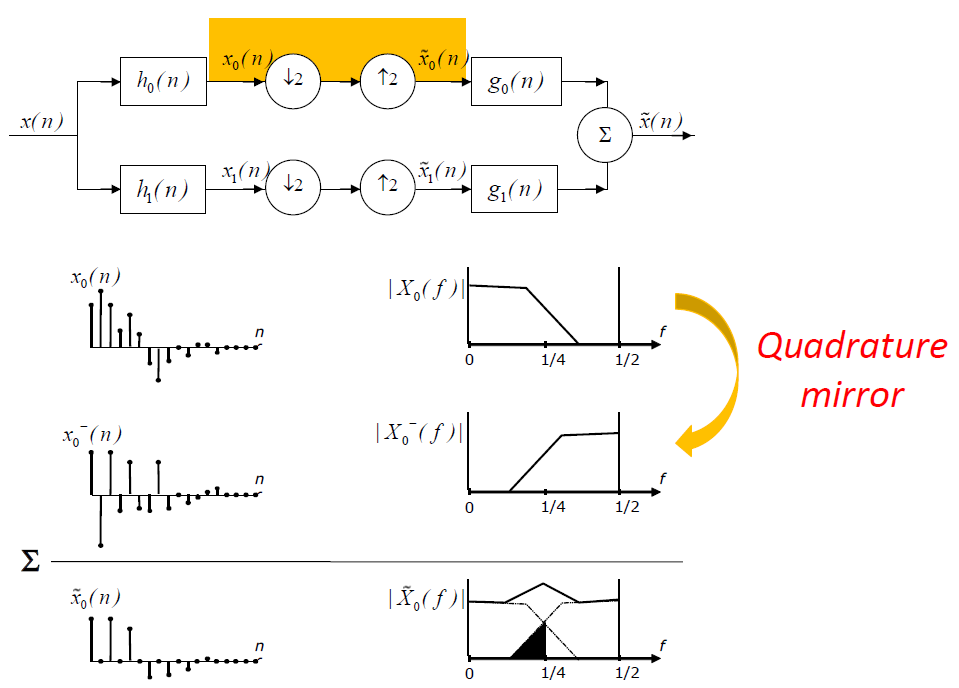
\includegraphics[width=5.5in]{Images/quadrature}
				\end{center}
				\begin{center}
					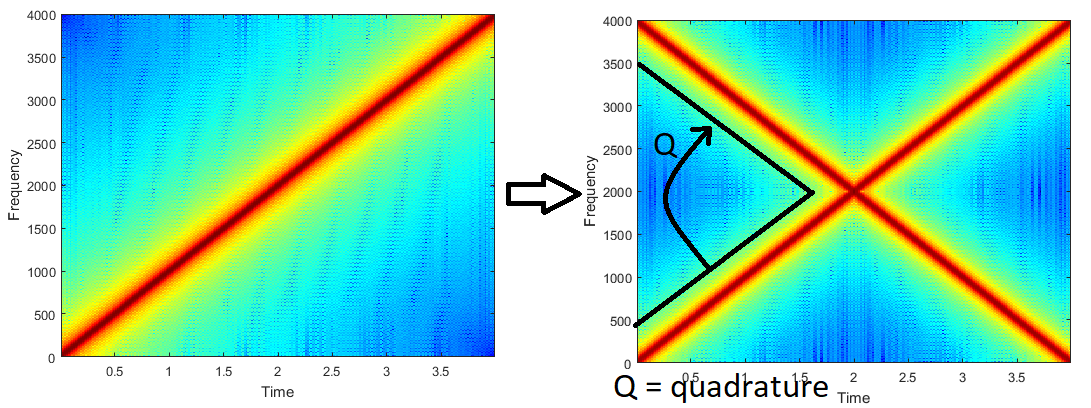
\includegraphics[width=4.5in]{Images/chirp}
				\end{center}
				On va alors faire en sorte que les filtres $g_0$ et $g_1$ produisent des \hl{recouvrements spectraux qui s'annulent} 
				réciproquement (Esteban \& Galland). Il y a plusieurs méthodes pour générer ces filtres. \hl{MP3 est un mélange de PQMF et 
				de MDCF}. En particulier, le MP3 effectue 32 fois moins de calcul que le MDCF car il calcule les cas particuliers 
				seulement.
			%
			\subsubsection*{Deux filtres simples}
				\alinea Dans l'exemple avec le chirp (On prend H0 = G0 et H1 = G1), 
					on a $M=2$. On a donc deux bandes : une passe-bas et une passe-haut. Les filtres H sont
					appelés filtres "quarter-band" et permettent de supprimer l'aliasing.
				%
				\begin{center}
					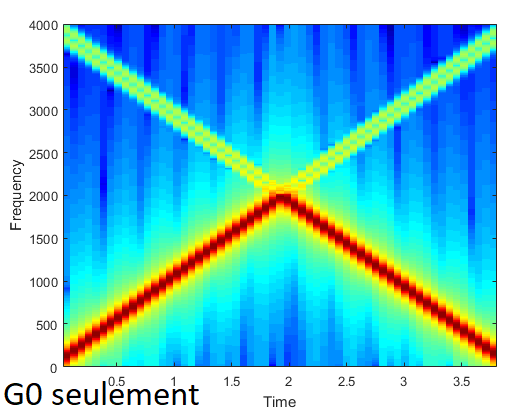
\includegraphics[width=1.5in]{Images/g0} \hfill 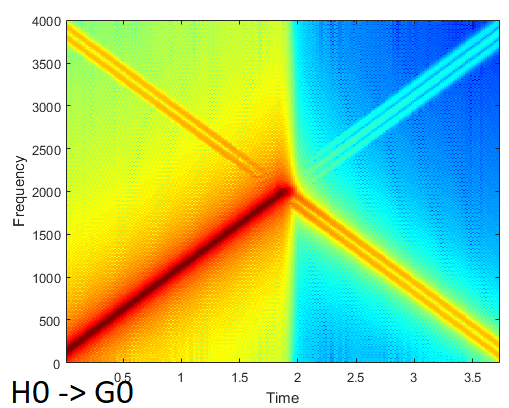
\includegraphics[width=1.5in]{Images/g0-and-h0} \hfill
					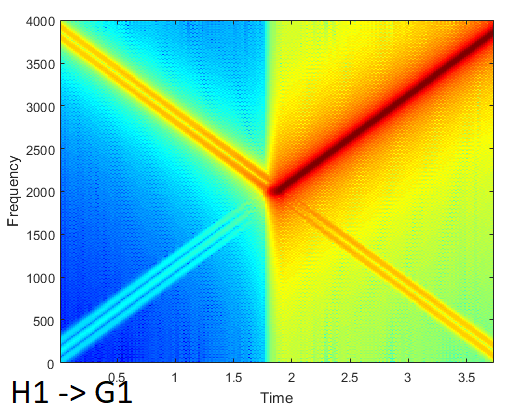
\includegraphics[width=1.5in]{Images/g1-and-h1} \hfill 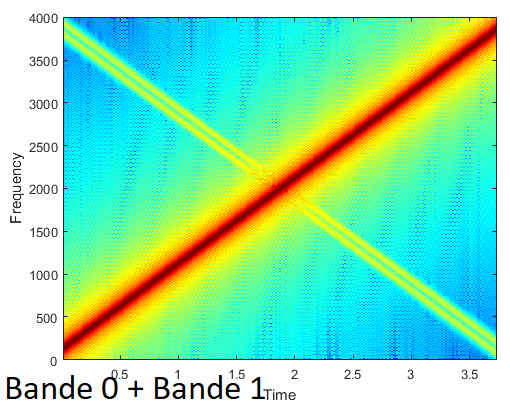
\includegraphics[width=1.5in]{Images/reconstruct}
				\end{center}
				%
			%
			\subsubsection*{Banque de filtres QMF}
				\alinea Ces filtres garantissent une reconstruction parfaite, tout en acceptant de l'aliasing dans les bandes.
					le fait d'additionner l'aliasing de chaque bande à la fin permet une annulation complète de l'aliasing.
				%
				\begin{center}
					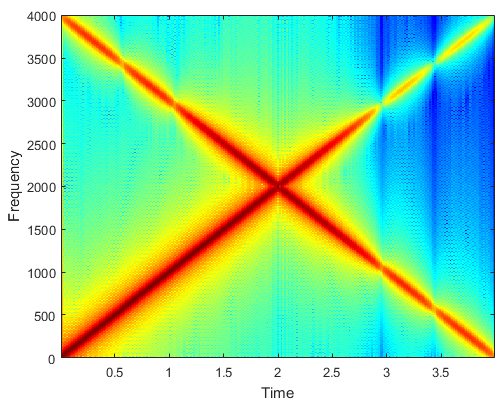
\includegraphics[width=2in]{Images/qmf1} \hfill 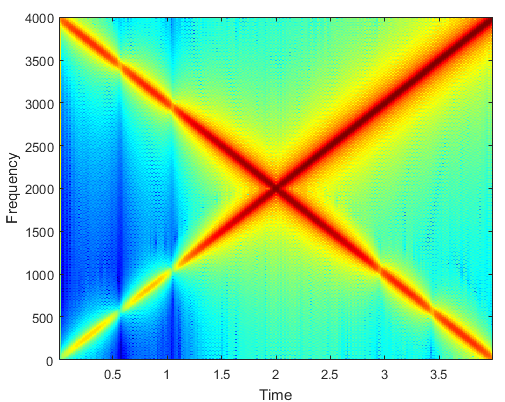
\includegraphics[width=2in]{Images/qmf2} \hfill
					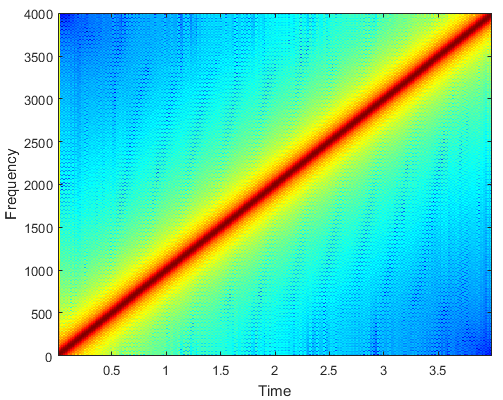
\includegraphics[width=2in]{Images/qmf3}
				\end{center}
				%
			%
		%
		\subsection{Encodage perceptuel}
			\alinea Lorsqu'on encode un signal sur un certain nombre de bit, l'erreur d'encodage peut être élevé. On peut
				baisser cette erreur en mettant des poids sur les sous-bandes de fréquence. En effet, on va utiliser l'amplitude
				(en valeur absolue) maximum afin de trouver le 'niveau de précision' nécessaire à l'encodage de cette bande de fréquence.
				On retrouve dans les exemples suivants : 1) un encodage typique sur 4 bits, 2) un encodage pondéré sur 4 bits, 3)
				un encodage pondéré sur 4 bits où les poids ont été multipliés par 10. \\
			%
			\alinea Si on divisait les poids par $x$, on augmenterait la précision de l'encodage, mais on couperait les hautes amplitudes
			(on considèrerait que le max des amplitudes est lui aussi divisé par $x$).
			%
			\begin{center}
				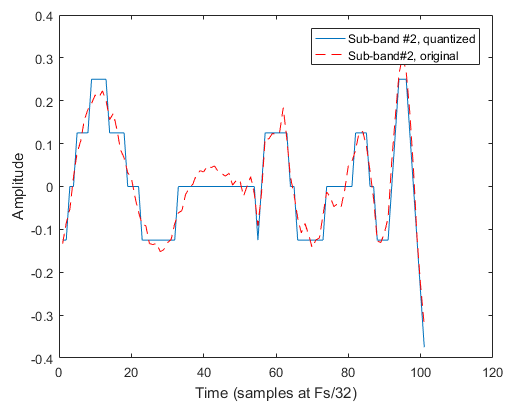
\includegraphics[width=2in]{Images/quantization1} \hfill 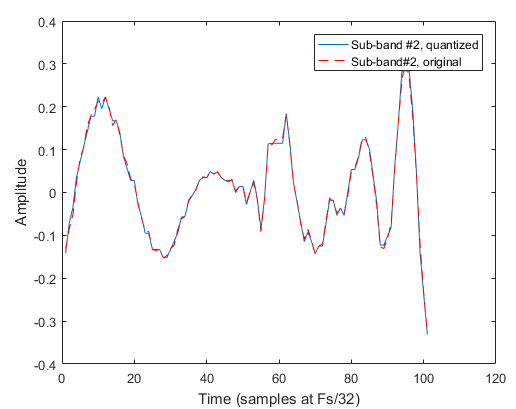
\includegraphics[width=2in]{Images/quantization2} \hfill 
				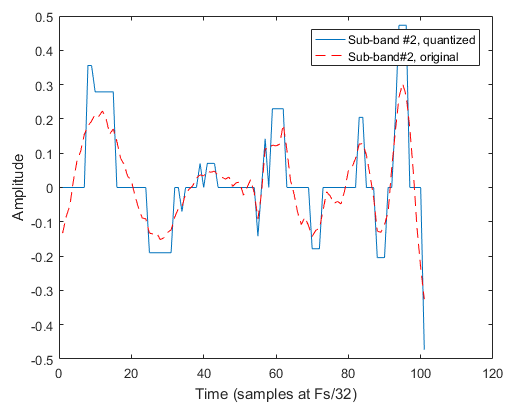
\includegraphics[width=2in]{Images/quantization3} 
			\end{center}
			%
			\alinea Le principe du MP3 est d'appliquer un tel encodage pondéré, en utilisant un modèle perceptuel calculé selon 
				l'oreille humaine. On va donc accentuer la précision sur les zones où l'oreille humaine est sensible et
				diminuer la précision dans les zones que l'oreille humaine n'entend pas. On dit donc que \hl{le signal sur bruit (SNR)
				doit rester au dessus du SMR} (seuil défini par le modèle auditif).
			%
			\begin{center}
				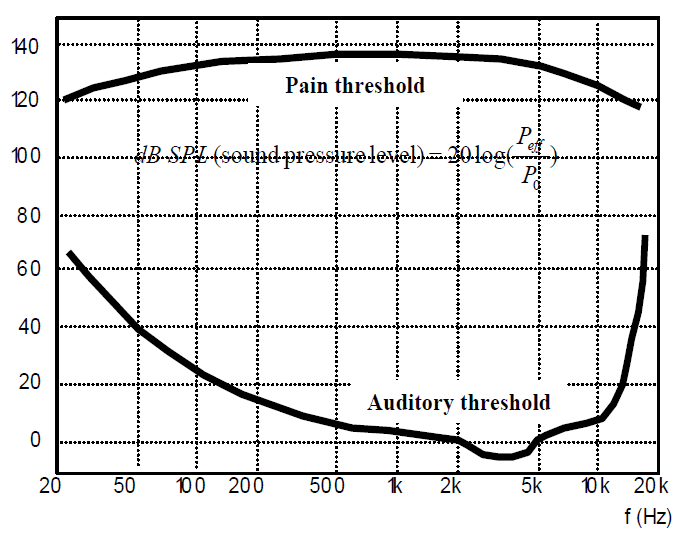
\includegraphics[width=3in]{Images/perceptual1} \hfill 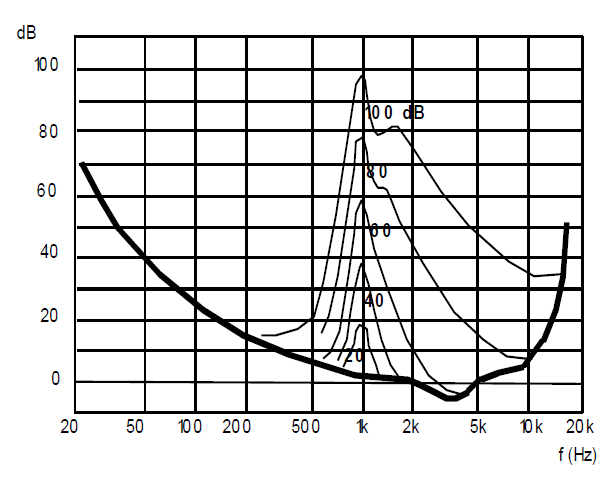
\includegraphics[width=3in]{Images/perceptual2}
			\end{center}
			%
		%
	%
	\section{Watermarking}
		\subsection{Principe général}	
			\alinea Le principe du watermarking va être d'utiliser une encodage en \red{spread spectrum} classique, comme celui de l'ADSL 
				sur le signal téléphonique, afin de cacher une information ou un message dans un signal audio. Pour ce faire,
				on va considérer \hl{le signal audio comme étant le bruit}, et la watermark comme étant le signal d'origine.
			%
		\subsection{Spread spectrum}
			\alinea On commence donc par encoder un message en bits. Ensuite, on va générer un "spread signal" qu'on utilisera pour
				encoder le message dans le signal audio (qui est considéré comme le bruit). En effet, ce faisant, on peut
				rendre la densité spectrale de puissance plus plate, et donc mieux faire passer 'incognito' la watermark dans le son.
				Il reste alors à additionner le signal audio avec la watermark pour donner le son "watermarké".
				Le nombre d'échantillons pris par le spread signal est calculé grâce à $\frac{Fs}{debit}$). Pour démoduler,
				il faut alors multiplier les frames (autant de fois qu'il y a de bits dans le message) du son watermarké par 
				le spread signal. 
				\begin{center}
					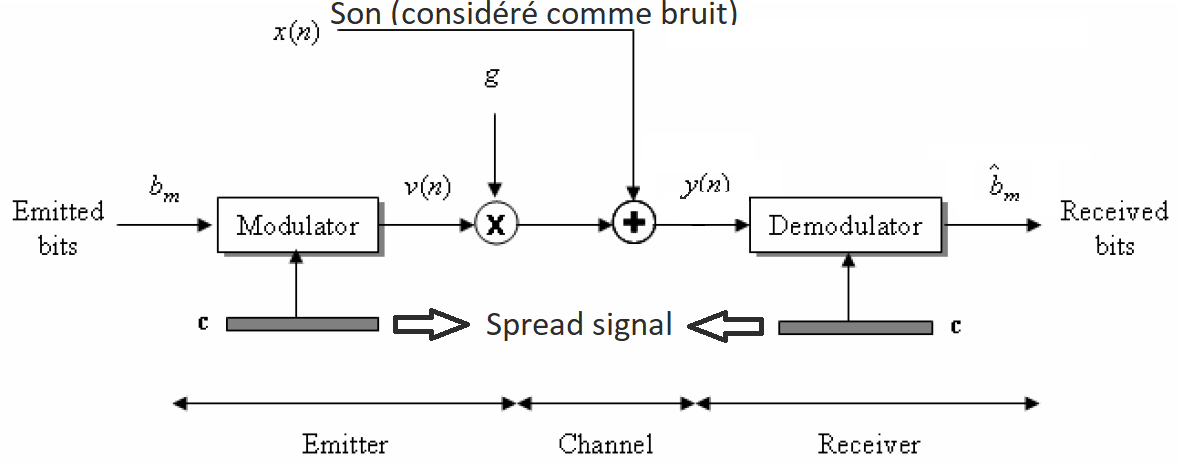
\includegraphics[width=6in]{Images/watermark}
				\end{center}
				\begin{center}
					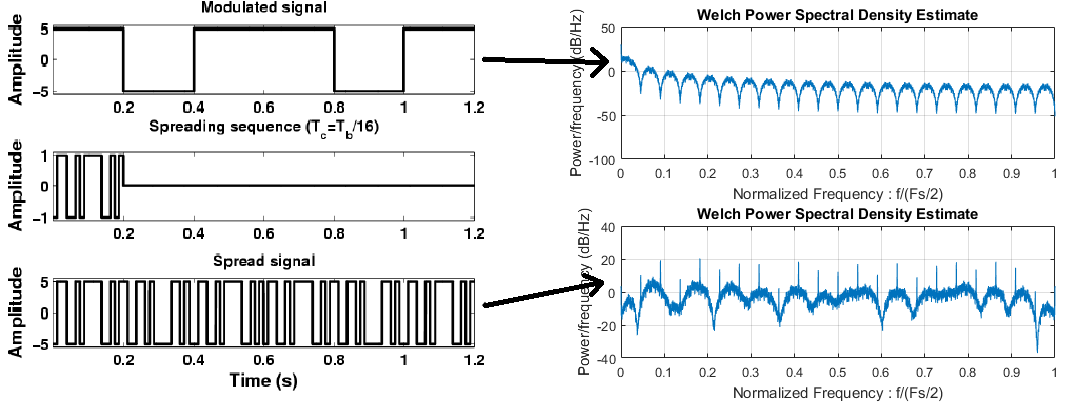
\includegraphics[width=6.5in]{Images/watermark-psd}
				\end{center}
			%
		%
		\subsection{Minimiser l'erreur}
			\alinea En \hl{augmentant le gain (et donc le SNR)}, on réduit l'erreur, mais on augmente aussi l chance d'entendre 
				la watermark. De plus, en \hl{diminuant le débit}, on peut également réduire l'erreur (réduire la zone de confusion 
				entre les gaussiennes).
			%
			\begin{center}
				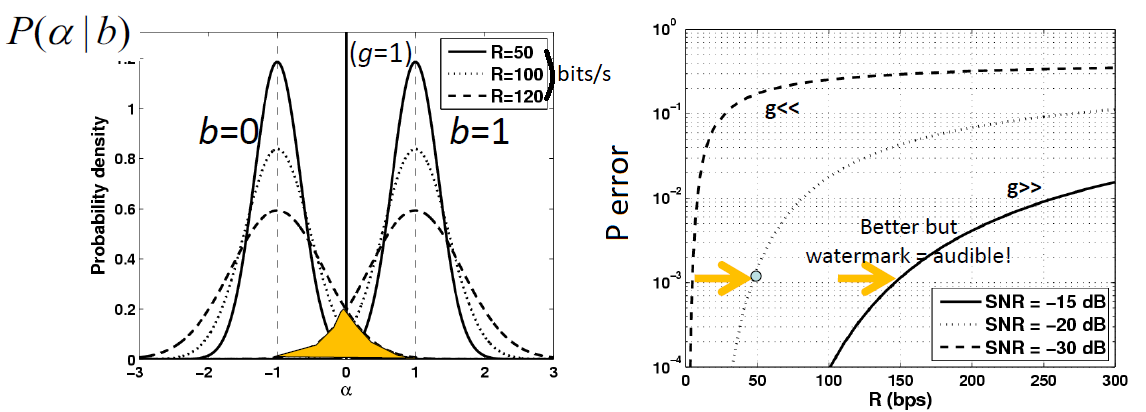
\includegraphics[width=5.2in]{Images/watermark-error}
			\end{center}
			%
			\alinea L'idée est donc de réduire le débit autant que possible, en poussant le gain un minimum. En particulier, on peut
				\hl{augmenter le gain "juste ce qu'il faut"} pour ne pas avoir d'erreur de détection. Mais de cette manière, on risque
				très probablement d'entendre la watermark au dessus de l'audio...
			%
			\begin{center}
				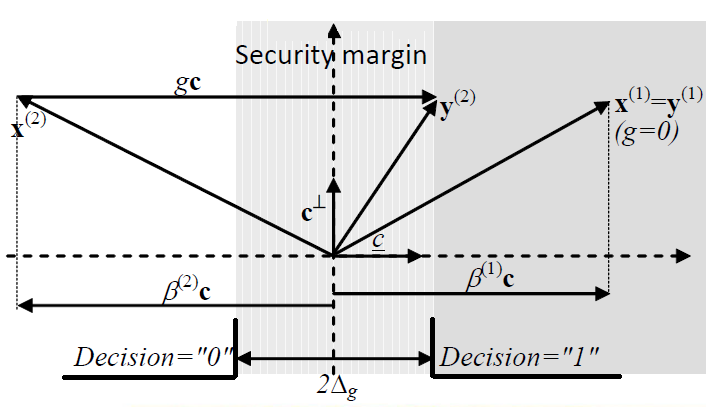
\includegraphics[width=3.2in]{Images/watermark-security}
			\end{center}
		\subsection{Modèle sycho-acoustique}
			\alinea On va donc utiliser le \hl{modèle psycho-acoustique} (PAM) pour augmenter le gain sur certaines bandes de fréquences
				inaudibles. On va donc pousser le gain par bande de fréquence, jusqu'à atteindre la limite audible. Ceci se fait grâce 
				à un \hl{"shaping filter"} (G) qui va faire coller la watermark au maximum au modèle auditif. Enfin, on a besoin
				d'un \hl{filtre de Wiener} (H) qui va extraire la watermark du signal encodé. H est un filtre tous zéros (non-récursif),
				et ses coefficients sont symétriques (filtre non-déphasant). 
			%
			\begin{center}
				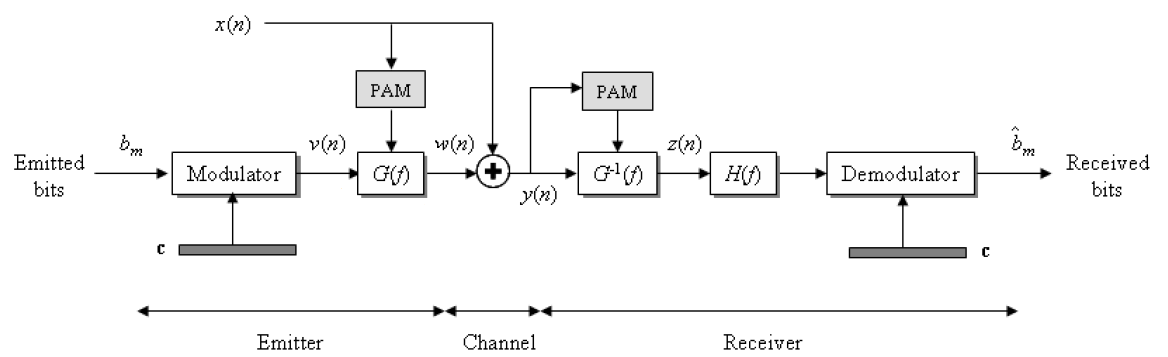
\includegraphics[width=6in]{Images/watermark-final}
			\end{center}
			%
			\alinea Pour calculer H, on aurait idéalement besoin de connaître v, mais si on connaît v, ça ne sert à rien de démoduler le
				signal... On va donc \hl{utiliser le spread spectrum pour estimer $\Phi_{\text{v v}}$.}
			%
			\begin{center}
				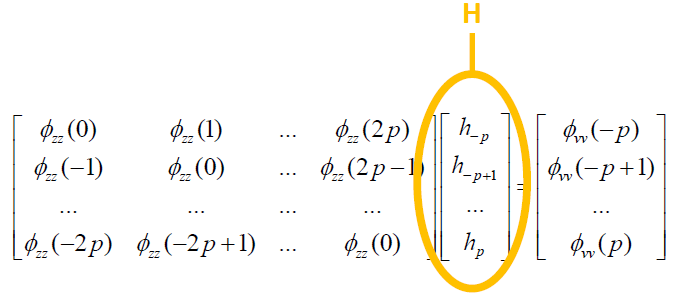
\includegraphics[width=4in]{Images/watermark-h}
			\end{center}
			%
		%
	%
	\pagebreak
	%
	\section{Dictation machine}
		\subsection{Principe général}
			\alinea Le principe ici est de calculer les probabilités d'obtenir des séquences de lettres. Formalisé, ça donne ceci :
			%
			\begin{center}
				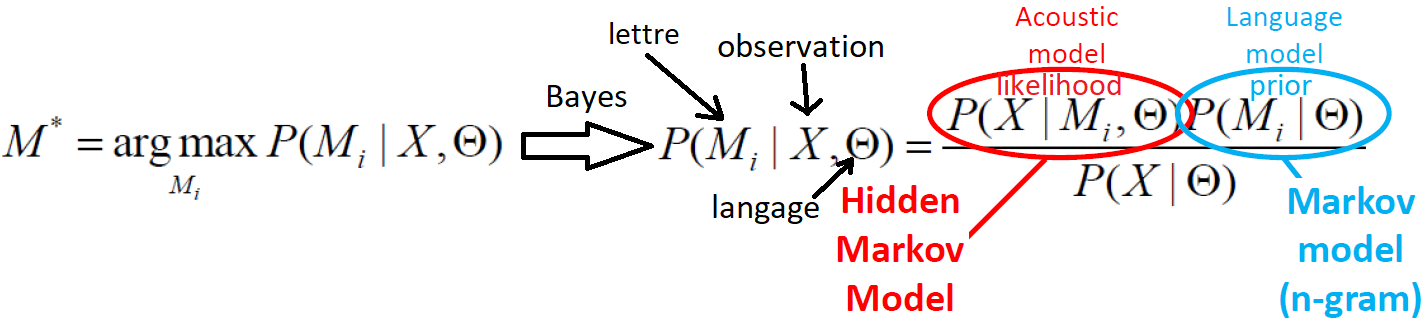
\includegraphics[width=4.25in]{Images/dictation}
			\end{center}
			%
			\alinea On peut alors essayer de retrouver la lettre en fonction des fréquences détectées (et donc par leurs formants)
				et éventuellement en fonction des lettres précédentes. On fonctionne généralement avec le \hl{logarithme des probabilités
				afin d'avoir des nombres plus grands et plus comparables}
			%
		%
		\subsection{Approche statique}
			\begin{minipage}{0.75\textwidth}
				\alinea Cette première approche suppose que l'ordre temporel des lettres n'a pas d'importance. C'est évidemment faux,
				mais cela peut servir à introduire le sujet. On commence alors par calculer les \hl{probabilités a priori} ($P(X)$) des
				lettres (probabilités de tomber sur la lettre $X$) en fonction du jeu de données. Ensuite, il reste à calculer les 
				'likelihood' de chaque observation en fonction de chaque lettre. Ceci peut se faire grâce à un modèle gaussien.
			\end{minipage}\hfill
			\begin{minipage}{0.2\textwidth}
				\begin{center}
					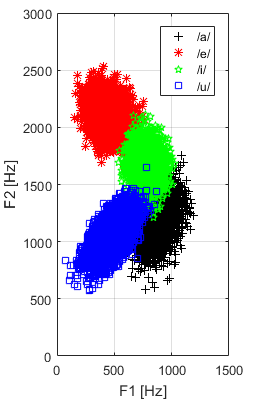
\includegraphics[width=\textwidth]{Images/dictation-formants}
				\end{center}
			\end{minipage}
			%
			\begin{minipage}{0.4\textwidth}
				\begin{center}
					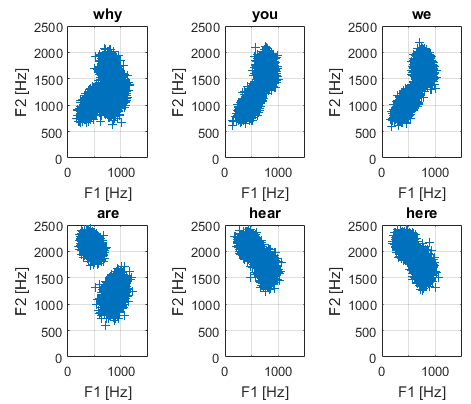
\includegraphics[width=\textwidth]{Images/dictation-gmm}
				\end{center}
			\end{minipage}\hfill
			\begin{minipage}{0.55\textwidth}
				\alinea Comme chaque lettre peut être représentée par une gaussienne, des mots peuvent être représentés par un modèle
					de mélange de gaussiennes. Ce genre de modèle posera \hl{problème lorsque l'ordre des lettres à de l'importance}. 
					Dans l'exemple, les mots 'you' (/iu) et 'we' (/ui) auront exactement le même modèle, et on ne pourra donc pas les
					distinguer avec une telle approche. 
				%
			\end{minipage}~\\~\\~\\
			%
			\alinea On peut estimer un tel modèle grâce à un clustering (il faut prendre des valeurs réelles, où proche de celles-ci
				pour initialiser k-means). Le problème est que \hl{k-means n'a qu'un sens géométrique}. On va faire appel à l'algorithme
				d'\hl{Estimation-Maximisation} (E-M) avec les valeurs obtenues par k-means comme valeurs initiales.
				Estimation = On calcule les probabilité pour une donnée d'appartenir à un modèle (cluster). Maximisation = On
				recalcule les moyennes/variances pour maximiser la séparation entre les classes.
			%
		%
		\subsection{Approche séquentielle}
			\subsubsection*{HMMs}
				\alinea On va utiliser ici des modèles de Markov cachés. Ces modèles sont des machines à états qui ont des probabilités
					d'émission et de transition. Les probabilités de transitions sont nécessaires pour passer d'un état à un autre.
					On va alors chercher le "best-path" parmi les modèles de Markov disponibles en utilisant l'algorithme de \hl{Viterbi}.
				%
			%
			\subsubsection*{N-grams}
				\alinea On va utiliser des probabilités que deux mots puissent se suivre. Par exemple, pour séparer 'hear' (/ir) et 'here'
					(/ir), qui ont la même prononciation, on peut dire que le bigram ('we', 'here') est très peu probable. 
					On peut calculer ces probabilités sur de grandes bases de données de phrases.
				%
			%
		%
	%
%
\pagebreak
%
\part{Dupont -- Reconnaissance automatique}
	\section{Introduction}
		\subsection{Analyse / Reconnaissance}
			\alinea Il y a deux étapes dans la reconnaissance automatique de sons : 
			\begin{itemize}
				\setlength\itemsep{0cm}
				\item \red{Analyse} -- Extraction d'\hl{attributs} (features) et d'\hl{information haut-niveau depuis un signal brut}.
				\item \red{Reconnaissance} -- \hl{Utilisation des attributs} extraits par l'analyse pour \hl{reconnaître/classer} un son, 
					une musique.
			\end{itemize}
			%
			\alinea Depuis l'arrivée des réseaux de neurones profonds, ces étapes tendent à se confondre (à cause des CNNs qui analysent
				et classent). Si on regarde la musique comme un signal temporel uniquement, c'est un \hl{signal très désordonné} et est 
				un peu un fouillis. Le but de l'analyse/reconnaissance c'est d'arriver à \hl{analyser les sons et les musiques comme 
				le cerveau humain} le ferait : isoler des instruments, isoler le rythme et le tempo, imaginer une partition musicale
				permettant de jouer la musique écoutée, ...
			%
		%
		\subsection{Domaines d'application}
			\begin{itemize}
				\setlength\itemsep{0cm}
				\item \red{Identification de musiques} -- Reconnaître artiste et titre d'une musique.
				\item \red{Transcription de musiques} -- Extraire la partition d'une musique. Les machines en sont actuellement 
					incapable, mais la recherche se focalise sur des sous-problèmes comme identifier les instruments joués, le rythme, etc...
				\item \red{Recommandation de musiques} -- Trouver des similitudes entre les musiques pour proposer des playlist.
				\item \red{Production de musiques} -- Modifier des sons pour améliorer la qualité de la musique ou générer des effets.
			\end{itemize}
			%
		%
		\subsection{Structure musicale}
			\alinea Au niveau de l'analyse, on peut établir une hiérarchie concernant les parties de musiques analysées.
				La \hl{plus petite partie} analysable d'un fichier audio est une \hl{trame (frame) audio}. 
				A partir de celles-ci, on peut établir une hiérarchie allant du plus gros agglomérat à la plus petite partie audio : 
				$$ \text{Sections} \Rightarrow \text{Mesures} \Rightarrow  \text{Beats} 
				        \Rightarrow \text{Segments} \Rightarrow \text{Trames} $$
				Ce qui veut dire qu'on peut former un segment à partir de plusieurs trames, un beat à partir de plusieurs segment, etc...
				On peut noter qu'un \red{segment} \hl{représente une note, de son début à sa fin}.
			%
		%
		\subsection{Dimensions musicales}
			\alinea \hl{Trois dimensions principales} peuvent être isolées en parlant de musiques 
				(avec les outils permettant de les analyser) : 
			%
			\begin{itemize}
				\setlength\itemsep{0cm}
				\item \red{Le timbre du son} -- MFCCs.
				\item \red{La mélodie, l'harmonie, les accords} -- Chroma
				\item \red{Le rythme et le tempo} -- Rythmogramme
			\end{itemize}
			%
			Ces trois dimensions seulement ne suffisent pas pour décrire les musiques les plus complexes.
			%
		%
	% 
	\section{Analyse musicale} 
		\subsection{Reconnaissance locale}
			\subsubsection{Timbre}
				\alinea Le \red{timbre} représente \hl{tout ce qui rend le son particulier}. Par exemple la différence entre une note 
					de piano et la même note jouée à la guitare est le timbre du son. On parle aussi de timbre pour des combinaisons 
					d'effets différents. On utilise des Mel-frequency cepstral coefficients (\hl{MFCCs}) sur chaque frame comme attributs 
					du son pour isoler le timbre. En effet, \hl{les MFCCs sont utilisés car ils ne prennent pas en compte le "pitch"}, 
					et donc la note jouée. En pratique, on
					utilise un \red{timbregramme}, qui est une \hl{séquences de MFCCs} affichée de manière similaire à un spectrogramme. 
					Ils sont une \hl{représentation compacte de l'enveloppe spectrale de puissance}. L'idée est que \hl{chaque coefficient 
					représente une partie du timbre}.\\
				%
				~\\
				%
				\alinea Les MFCCs sont bons pour détecter les \hl{instruments utilisés}, mais aussi pour détecter \hl{l'artiste} et 
					\hl{le genre}. En effet, les effets utilisés peuvent aider pour classifier le genre, et les instruments utilisés 
					peuvent aider à reconnaitre l'artiste.
				%
			%
			\subsubsection{Harmonie}
				\alinea Pour détecter les harmonies et les notes en général, on va utiliser des \red{chromagrammes} sur des 
					frames de musique (30ms). Ils vont tenter de 
					\hl{détecter des suites de notes en ignorant l'octave de ces dernières}. De cette manière, on peut \hl{identifier les
					accords joués} (ainsi que leurs variantes: mineurs, 7$^{\text{\`eme}}$, ...). Le principe est qu'une banque de filtres
					et utilisée afin d'isoler chaque note. Pour chaque note, un \hl{filtre $B(x)$} est utilisé et retourne 1 si le modulo 12 
					vaut 0 (si on se trouve à une \hl{octave de la note du filtre}). On peut noter que dans la formule, un paramètre $k_0$
					permet d'accorder le chroma à sa guise (pour varier du La à 440Hz par exemple).
				%
				\begin{center}
					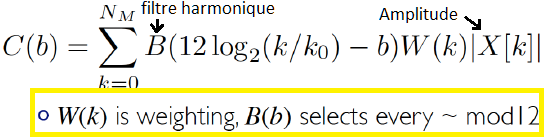
\includegraphics[width=3in]{Images/chroma-eq} \hfill 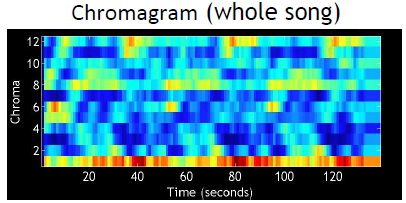
\includegraphics[width=3in]{Images/chroma}
				\end{center}
				%
				\alinea Le chromagramme tel quel a un problème : il \hl{dépend de la précision de la FFT utilisée}. En effet, les fréquences
					(discrètes) détectées par la FFT peuvent être un peu décalées par rapport aux fréquences des notes de musique.
					Le chromagramme peut être utilisé pour reconnaître les accords, la clé de la musique, les émotions données par la musique,
					ou encore pour analyser les musiques qui vont bien ensemble (utilisent la même suite d'accord).
				%
			%
			\subsubsection{Rythme}
				\alinea Contrairement aux deux précédentes dimensions, \hl{le rythme s'analyse sur plusieurs secondes de musique}, un 
					beat n'a de sens qu'avec les beats qui l'entourent pour finalement former un rythme. C'est pourquoi on va 
					\hl{analyser des mesures}.
				%
				\begin{center}
					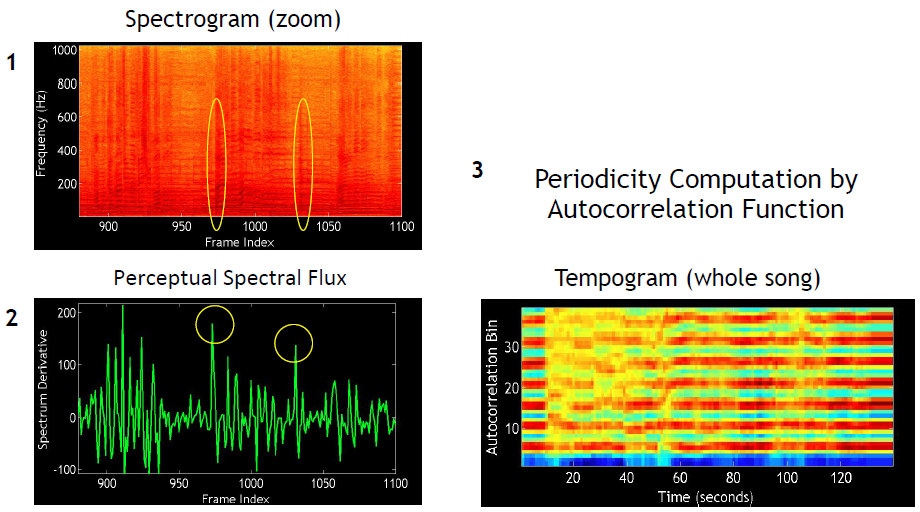
\includegraphics[width=5.2in]{Images/tempo} 
				\end{center}
				\begin{center}
					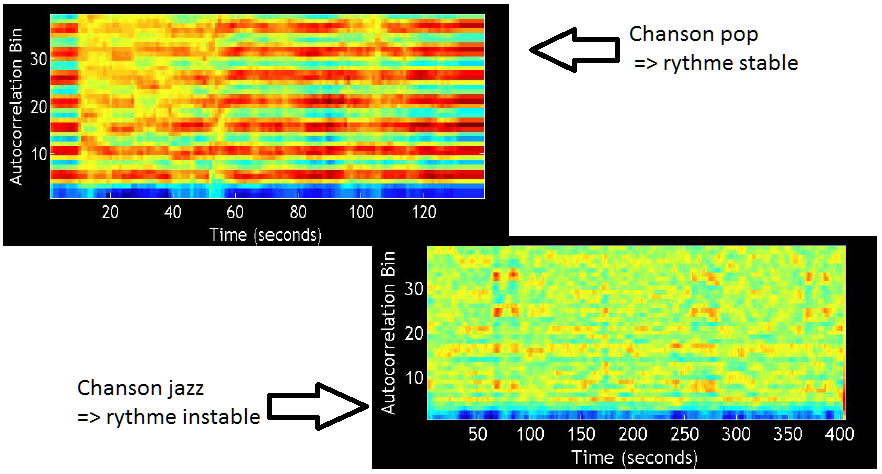
\includegraphics[width=4.66in]{Images/tempo2}
				\end{center}
				%			
				\alinea Le \hl{flux spectral perceptuel} représente un graphe de changement local. A chaque pic, on dit qu'il y a un 
					\hl{nouvel "event"}. C'est pourquoi les parties de chanson avec une batterie forte présentent des pics réguliers et 
					donc un tempogramme régulier. Il y a plusieurs lignes à cause des multiple de la période (genre 2$\pi$, 4$\pi$, ...). 
					Pour rectifier le tir, on va utiliser un \hl{tempogramme cyclique} dont les ordonnées $\in [1, 2]$ car on retient tout 
					ce qui se trouve entre le tempo de base (1) et ses multiples (2).
				%
				\begin{center}
					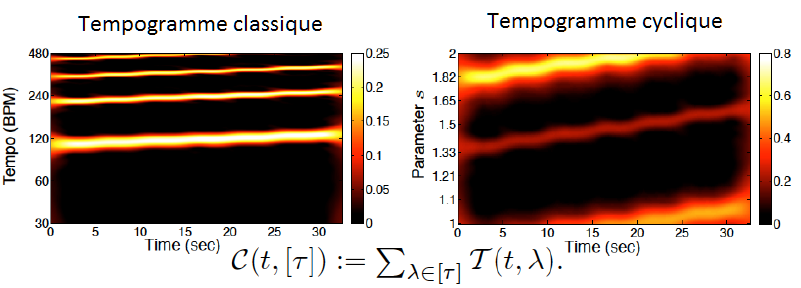
\includegraphics[width=5in]{Images/tempograms}
				\end{center}
				%
				\alinea On peut utiliser les tempogrammes pour \hl{segmenter les musiques} en différentes parties. On peut imaginer 
					qu'à chaque changement de rythme, une nouvelle partie de la musique commence
				%
				\begin{center}
					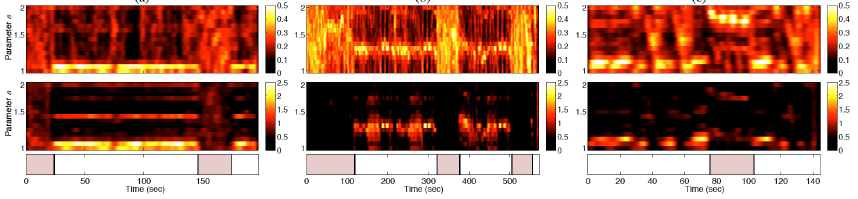
\includegraphics[width=\textwidth]{Images/segmentation}
				\end{center}
				%
			%
			\subsubsection{En bref}
				\alinea Grâce au timbre (timbregramme), aux notes (chromagramme) et au rythme (tempogramme), on peut essayer de classer
					des musiques selon leur genre et selon les émotions qu'elles évoquent.
				%
				\begin{center}
					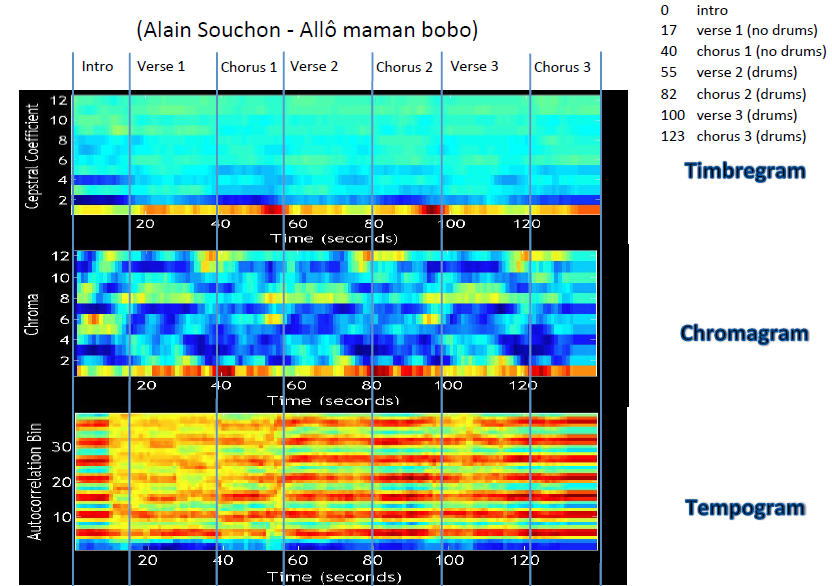
\includegraphics[width=5in]{Images/local_summary}
				\end{center}
				%
			%
		%	
		\subsection{Débuts de segment (onset)}	
			\alinea Cette partie est consacrée au calcul du flux spectral perceptuel. En effet, on a besoin de \hl{détecter le début de chaque
				note jouée} pour pouvoir estimer le début d'un nouvel "event". Cela pose \hl{quelques problèmes à résoudre} : 
				\begin{itemize}
					\setlength\itemsep{0cm}
					\item Séparer les notes de plusieurs instruments qui jouent en même temps.
					\item Combler le manque de démarcation claire (note qui change sans impulsion claire).
					\item Ne pas considérer un arrêt soudain d'une note comme un nouvel "event".
				\end{itemize}
			%
			\alinea La création de la fonction de détection d'onset (onset strength function) s'appelle aussi la \hl{réduction} car on 
				part d'un signal audio complet pour obtenir un signal réduit ne comprenant que des probabilités d'avoir un onset à un 
				moment donné (car on va avoir une valeur toutes les 10ms environs, donnant une fréquence de 100Hz).\\
			%
			\begin{minipage}{0.55\textwidth}
				\alinea Il y a trois chose que l'on peut faire pour la partie "réduction".
				\begin{itemize}
					\setlength\itemsep{0cm}
					\item Détecter les changements temporel (saut d'énergie soudain).
					\item Détecter les changements spectraux (changements nets dans des fft sur de courtes périodes).
					\item Utiliser des modèles probabilistes.
				\end{itemize}
			\end{minipage} \hfill
			\begin{minipage}{0.35\textwidth}
				\hl{\ \ \ \ \ \ \ \ \ \ \ \ \ \ \ \ \ \ \ \ \ \ \ \ \ \ \ \ \ \ \ \ \ \ \ \ \ \ \ \ \ \ \ \ \ \ \ \ \ \ \ \ \ \ \ \ \ \ }
				\begin{center}				
					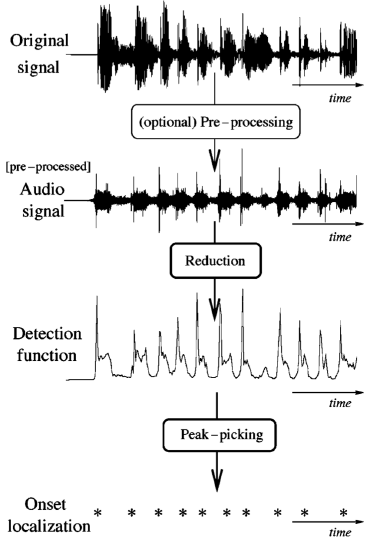
\includegraphics[width=\textwidth]{Images/onset}
				\end{center}
				\hl{\ \ \ \ \ \ \ \ \ \ \ \ \ \ \ \ \ \ \ \ \ \ \ \ \ \ \ \ \ \ \ \ \ \ \ \ \ \ \ \ \ \ \ \ \ \ \ \ \ \ \ \ \ \ \ \ \ \ }
			\end{minipage}~\\~\\~\\
			%
			\subsubsection{Variation d'énergie}
				\alinea On ne peut pas toujours détecter les onset par la dérivée de l'énergie car les notes sont parfois toutes
					connectées
				%
				\begin{center}
					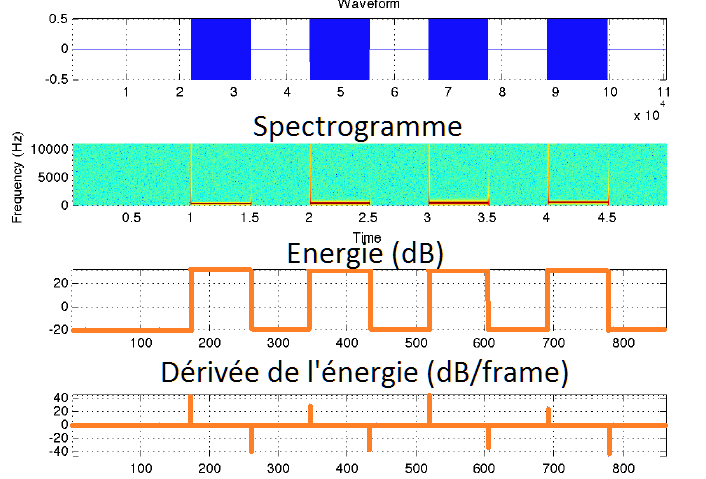
\includegraphics[width=0.49\textwidth]{Images/onset-ex} 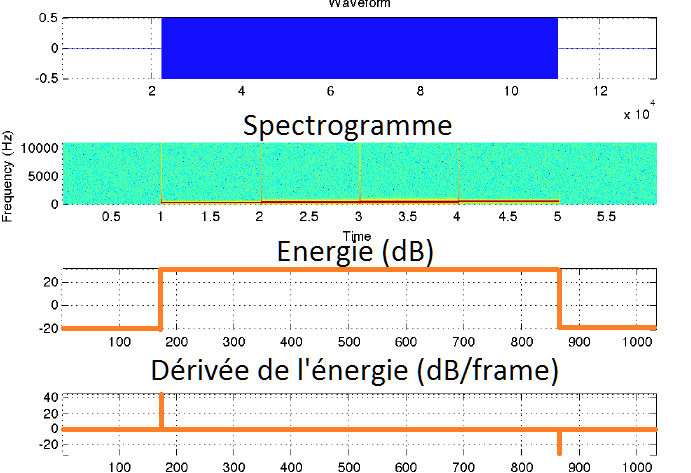
\includegraphics[width=0.49\textwidth]{Images/onset-ex2}
				\end{center}
				%
				\alinea Pour remédier à ce problème, on peut \hl{amplifier l'amplitude des hautes fréquences} dans le spectre afin de 
					marquer les changements abrupts. En effet, \hl{un changement soudain implique une montée d'énergie dans les hautes
					fréquences}. C'est ce qu'on a fait dans l'exemple suivant; on a calculé l'énergie sur le spectre amplifié en hautes
					fréquences. \\
				%
				\begin{minipage}{0.49\textwidth}
					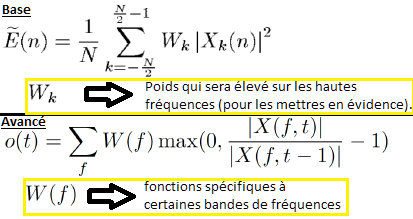
\includegraphics[width=\textwidth]{Images/onset-eq1}
				\end{minipage} \hfill
				\begin{minipage}{0.49\textwidth}
					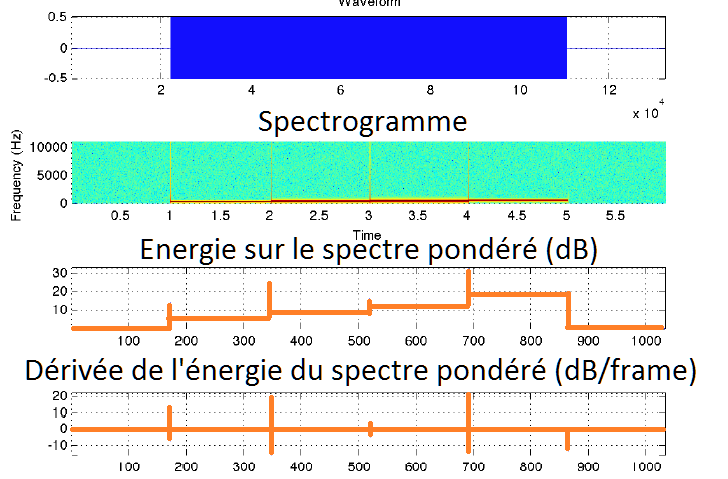
\includegraphics[width=\textwidth]{Images/onset-amplified}
				\end{minipage}
				%
			%
			\subsubsection{Variations spectrales}
				\alinea On va ici regarder les changements entre des FFT consécutives. On va donc faire la \hl{différences entre plusieurs
					FFT}. On ne \hl{garde que les différences positives} (et on retourne 0 sinon) car on cherche de nouvelles fréquences 
					( si nouvelle - ancienne > 0 alors il est possible qu'une nouvelle note soit jouée). On finit par trouver des 
					changements de fréquence fondamentale en accumulant ces différences pour chaque bande de fréquence.\\
				%
				\begin{minipage}{0.49\textwidth}
					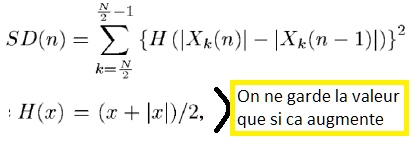
\includegraphics[width=3in]{Images/spectral-eq}
				\end{minipage} \hfill
				\begin{minipage}{0.49\textwidth}
					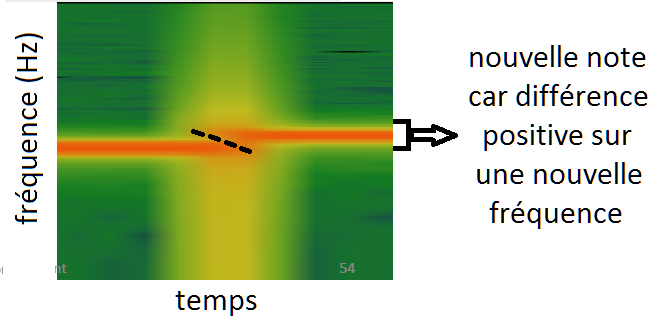
\includegraphics[width=3in]{Images/spectral}
				\end{minipage}~\\~\\
				%
				\alinea On a encore un problème à ce niveau-ci : Si un joueur de violon \hl{rejoue une même note}, on doit pouvoir détecter
					la nouvelle note, mais la différence spectrale n'y verra rien car ce seront presque les même composantes en fréquences 
					qui seront jouées. Par contre, on aura un \hl{changement de phase} car on recommence à jouer la note.\\
				%				
				~\\			
				%
				\alinea \hl{Une analyse trame par trame implique que la phase va changer à chaque analyse. Cependant, on peut prédire la phase
					de la prochaine analyse car elle augmente de manière linéaire jusqu'à retomber à zéro (évolution cyclique).}
					On va donc estimer qu'il y a une nouvelle note lorsqu'il y a \hl{un changement abrupt (non-linéaire, différent de la
					valeur prédite) de phase}. Tout ceci est illustré dans l'exemple suivant.
				%
				\begin{center}
					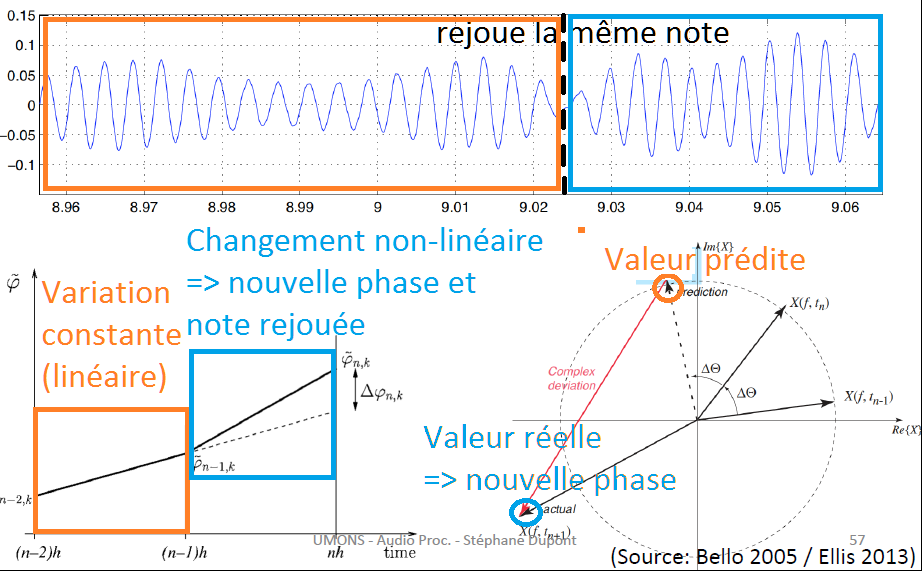
\includegraphics[width=\textwidth]{Images/phase}
				\end{center}
				%
				\alinea En pratique on a besoin de faire une analyse complexe de spectre dans la différence de fréquence et analyse de phase
					car sinon, la phase pourrait être trop sensible au bruit.
				%
			%
			\subsubsection{Sélection d'onset}
				\alinea Une fois que la fonction de détection d'onset est établie, il faut sélectionner les pics qui seront considérés comme
					onset, et donc comme début de segment. Ça peut se faire par une technique de \hl{sélection par seuil} ou par \hl{sélection
					intelligente de pic}. Cependant, un traitement supplémentaire est nécessaire avant de pouvoir faire cela. Un 
					\hl{post-traitement de la fonction de détection} est nécessaire afin de palier au changement d'orchestration de la chanson
					qui pourrait influencer la qualité des pics. On peut y appliquer un filtre passe-bas pour la lisser, un filtre passe haut 
					pour mettre en évidence les pics, on peut aussi la normaliser par l'écart-type, ...
				%
			%
			\subsubsection{\'Evaluation des performances}
				\alinea Deux méthodes sont utilisées en général pour évaluer les performances d'un détecteur : Précision/Rappel et la 
					F-mesure. La F-mesure valant $\frac{2 \cdot Precision \cdot Recall}{Precision + Recall}$
				%
				\begin{center}
					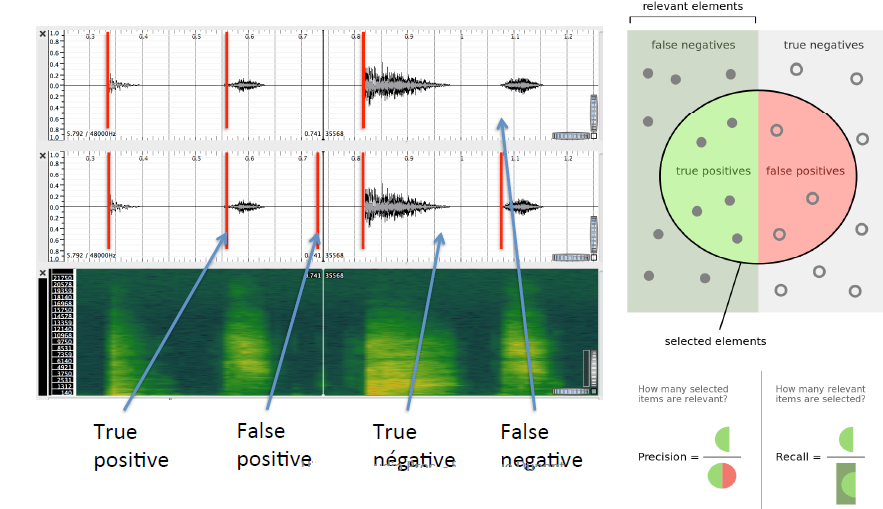
\includegraphics[width=\textwidth]{Images/precision}
				\end{center}
				%
			%
		%
		\subsection{Tempo}
			\alinea Jusqu'à présent, on s'est intéressé au rythme de manière locale, mais on voudrait maintenant avoir le \hl{tempo global} 
				de la chanson (e.g. 90BPM). Pour ce faire il faut détecter les onset. De plus, il faut s'intéresser aux "tatum", qui sont 
				des onsets entre les beats importants pour la perception. Typiquement, le \red{tempo} représente \hl{la périodicité entre 
				les onsets de grande intensité.}
			%
			\subsubsection{Méthode initiale}
				\alinea A la base, la recherche du tempo se faisait par \hl{recherche de fréquence}. On soumettait les onsets à des
					\hl{résonateurs}, qui cherchaient à quelle fréquence les résonateurs résonnaient le mieux. 				
				%
			\subsubsection{Approche d'auto-corrélation}
				\alinea On va chercher la\hl{ corrélation entre les onsets} en faisant glisser le graphe avec un certain délai à faire varier 
					(on superpose un onset avec tous les autres, mais décalés, pour connaître sa corrélation avec ceux là). 
					Le résultat donne les tempo possibles, mais avec les "octaves"
					possibles. C'est pourquoi on va pondérer le tout selon les tempo les plus utilisés en musique ou pour le genre musical en
					question (\hl{introduction de connaissance musicale}).
				%
				\begin{center}
					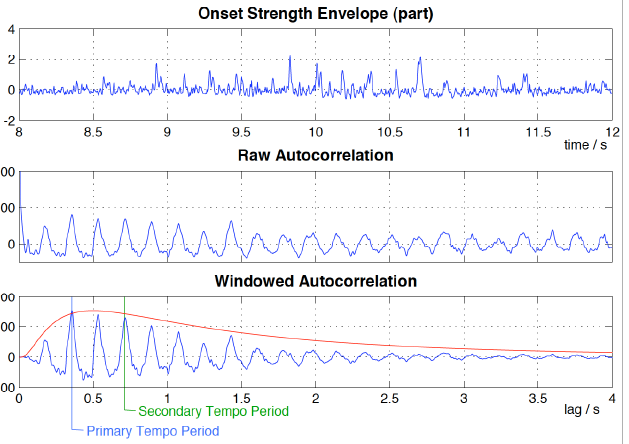
\includegraphics[width=5in]{Images/tempo3}
				\end{center}
				%
			%
		%
		\subsection{Beats}
			\alinea Une fois le tempo détecté, on peut s'attaquer à la détection des \red{beats} qui ne sont finalement que les 
				\hl{pics principaux d'onset séparés par des périodes de tempo}. Il faut donc chercher à \hl{maximiser la fonction}\\
				\begin{minipage}{0.5\textwidth}
					\begin{flushright}
						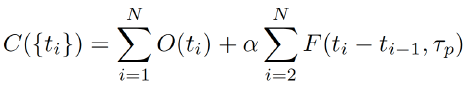
\includegraphics[width=0.75\textwidth]{Images/beat-eq}
					\end{flushright}
				\end{minipage} \hfill
				\begin{minipage}{0.49\textwidth}
					\begin{flushleft}
						$ = \text{onsets} + \alpha \cdot \text{régularité du tempo} $
					\end{flushleft}
				\end{minipage}~\\~\\~\\				
				$\alpha$ étant un facteur d'échelle, permettant de l'importance de la régularité du tempo. Le problème est que 
				cette fonction demande un temps exponentiel à maximiser. On va donc avoir recours à de la \hl{programmation dynamique}
				(stocker les résultats intermédiaires parce qu'ils se répètent dans les formules) afin de résoudre le problème
				de manière itérative. Une autre technique utilisée est de faire la corrélation des onsets avec un modèle collant au 
				tempo, avec une certaine tolérance à l'erreur.\\
			%
			~\\
			%
			\alinea Une chose plus compliquée à faire est de détecter les \red{downbeats}, qui sont les \hl{beats qui démarrent une mesure}.
				Pour ce faire, o\hl{n a besoin de plus de connaissances musicales} car sa position varie selon les genres musicaux.
				Des fonctions de signatures temporelles seraient nécessaires.
			%
		%
		\subsection{Conclusion}		
			\alinea Note générale sur l'analyse musicale: 
				\hl{Il y a beaucoup plus de techniques que celles vues au cours pour extraire des informations d'une musique.}
			%
		%
	%
	\section{Identification de musique}
		\alinea Principe : reconnaître une musique par son titre et artiste en n'écoutant que quelques secondes.
			Pour ce faire on va chercher une "empreinte digitale" unique pour la musique, qui pourra être reconnue en écoutant
			une partie de la musique.
		%
		\begin{center}
			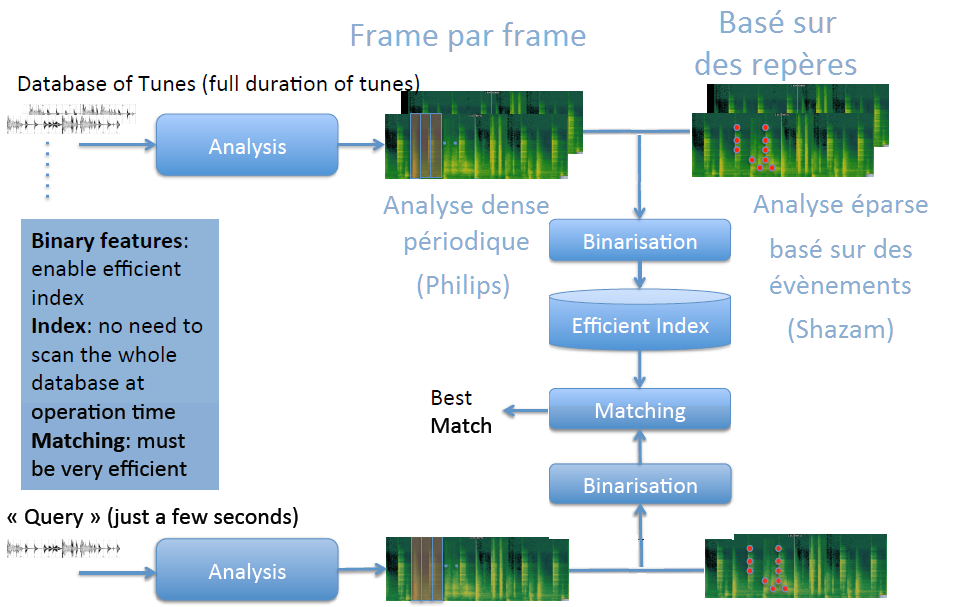
\includegraphics[width=6in]{Images/music_ID}
		\end{center}
		%
		\subsection{Analyse par frame}
			\alinea La méthode initiale consiste à \hl{encoder chaque frame sur 32 bits}. Les 32 bits représentent chacun une \hl{bande 
				de fréquence d'une FFT}. Pour chaque bande, s'il y a un \hl{changement local} conséquent par rapport à la FFT précédente, le 
				bit correspondant est mis à 1. Cette analyse se fait sur des frames plus longues que d'habitude ($\sim$100ms) afin 
				d'être plus \hl{robustes}.
			%
			\begin{center}
				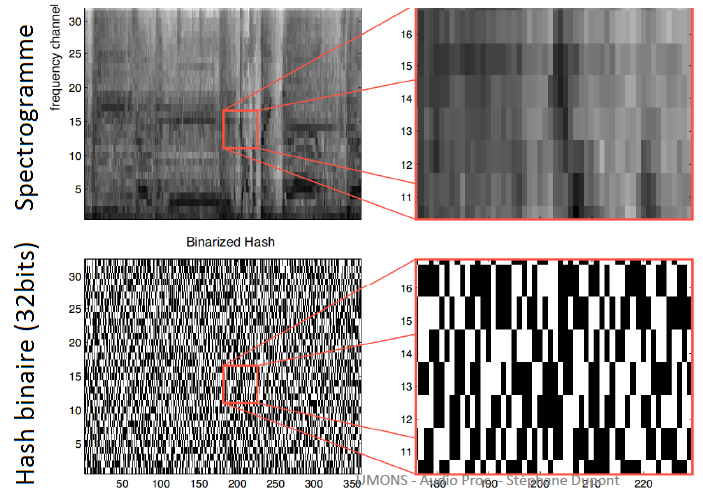
\includegraphics[width=3in]{Images/binary}
			\end{center}
			%
			\alinea On utilise ensuite ces 32 bits par frame pour retrouver la musique. La méthode principalement utilisée est une 
				"\hl{lookup table}" (LUT) qui a une table d'entrée contenant toutes les combinaisons possibles d'empreintes 32 bits
				($2^32$ possibilités). On a ensuite accès à n'importe quel endroit de n'importe quelle chanson et on peut 
				commencer à chercher un match.
			%
			\begin{center}
				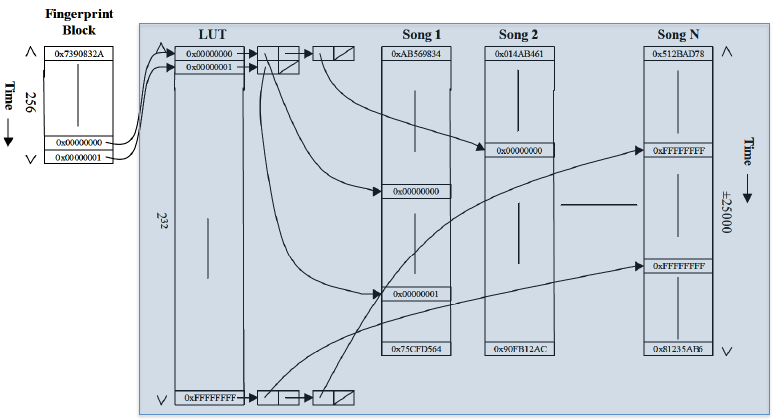
\includegraphics[width=\textwidth]{Images/LUT}
			\end{center}
			%
			\alinea En effet, utiliser une recherche en \hl{force brute est débile et prendrait trop de temps}. De plus, grâce à la LUT,
				on peut facilement contourner les \hl{erreurs à 1 bit près}. En inversant un par un les bits d'une séquence de 32 bits,
				on obtient 32 nouvelles séquences que l'on peut entrer dans la LUT. Néanmoins, \hl{le bruit peut poser problème} pour 
				retrouver correctement ces vecteurs 32 bits.
			%
		%
		\subsection{Analyse par repères (landmarks)}
			\alinea Le principe est de prendre un spectrogramme (fig. 1A), d'en \hl{extraire les pics}, et de se servir de chaque pic
				comme "\red{ancre}" (anchor) (fig. 1B). On va ensuite \hl{relier chaque ancre avec les autres pics (fig. 1C) et 
				former des triplets} \hl{(fréquence de démarrage, fréquence de fin, différence de temps)} (fig. 1D). Ce sont ces 
				triplets qui vont former nos repères dans la reconnaissance de musique. En pratique, on a pas besoin de trouver 
				beaucoup de landmarks communs pour identifier une musique.\\
			%
			~\\
			%
			\alinea Ces \hl{repères sont robustes} car ils se reposent sur les pics du spectrogramme qui sont les fréquences principales 
				et les harmoniques de celles-ci, et sont donc les \hl{composantes les plus fortes en énergie dans le spectre}. 
				Les valeurs des triplets sont discrétisées selon \hl{256 bandes de fréquences et 64 marquages temporels}.\\
				On a alors \hl{22 bits par repère} (fréquence, fréquence, temps) $\rightarrow$ (8 bits, 8 bits, 6 bits).
			%
			\begin{center}
				\includegraphics[width=\textwidth]{Images/landmark}
			\end{center}
			%
			\alinea La \hl{détection de pics dans le spectrogramme peut être ajustée} en réglant des paramètres afin de détecter moins ou plus 
				de pics, et ce afin de limiter le nombre de repères par chanson. Si de tels paramètres sont utilisés pour les chansons
				dans la base de données, alors ces paramètres doivent être appliqués également aux chansons écoutées (qui doivent être
				reconnues).\\
			%
			~\\
			%
			\alinea Ensuite, les repères sont présentés à une LUT qui va encore une fois retourner toutes les chansons qui contiennent
				le repère donné. Cependant,\hl{ pour reconnaître la musique, il va falloir faire appel au temps dans la chanson auquel 
				l'ancre du repère a été détecté}. En effet, on va faire une comparaison temporelle entre le moment où le (l'ancre du) 
				repère a été détecté et le moment ou le repère se trouve dans la chanson de la base de données.
				La comparaison devrait donner une séquence claire, permettant d'avoir un grand nombre de match sur une courte période,
				et donc un grand nombre de match dans un histogramme comptant le nombre de matchs par fenêtre de temps.
			%
			\begin{center}
				\includegraphics[width=5in]{Images/landmark2}
			\end{center}
			%
			\alinea Cette technique permet d'obtenir de \hl{très bon résultat, malgré un bruit élevé} (SNR de 3dB) et une compression
				élevée. Par contre, \hl{la technique est sensible à la modification de la vitesse} de la musique originale (car le repère 
				dépend du temps de par sa 3$^{\text{`eme}}$ composante) \hl{ou si on modifie le pitch de la musique} (car le repère dépend
				fortement des fréquences fondamentales).
			%
		%
	%
	\section{Réseaux de neurones (profonds)}
		\alinea Pour cette partie, c'est la reconnaissance vocale (ASR) qui va être étudiée. La technique de base pour faire de l'ASR
			consiste à suivre \hl{3 étapes} :
			\begin{enumerate}
				\setlength\itemsep{0cm}
				\item Extraire des informations utiles des fichiers audio (FFT, Spectrogramme, ...).
				\item Calculer les probabilités d'obtenir tel ou tel phonèmes à partir des informations extraites.
				\item Calculer les probabilités d'obtenir un tel mot ou une telle phrase selon une suite de phonèmes.
			\end{enumerate}
		%
		\alinea Les deux principales faiblesses de cette technique est (1) qu'il faut \hl{évaluer à la main l'utilité des informations} à
			extraire de l'audio \hl{pour chaque nouvelle tâche} et (2) qu'il n'y a \hl{pas d'optimisation globale} de ces 3 étapes, 
			il n'y a qu'une optimisation locale pour chaque étape. De plus, \hl{les performances n'égalent pas les performances humaines}.
			Pour remédier à ces problèmes, on va faire appel à des \hl{réseaux de neurones profonds qui vont effectuer les 3 étapes eux-même},
			permettant une optimisation globale et une facilité d'utilisation (car pas d'analyse des features intéressantes).
			Ce faisant, \hl{on se débarrasse de la partie analyse du signal}, mais aussi des \hl{suppositions} faites sur les 
			\hl{modèles probabilistes} et sur \hl{les features qui pourraient être intéressantes}.
		%
		\subsection{Neurone}
			\alinea Avant de créer un réseau, on va commencer par définir ce qu'est un neurone. Deux fonctions intéressaient les chercheurs 
				à la base : (1) \red{le symbolisme}, permettant de représenter les données et la connaissance humaine, et (2) 
				\red{le connectionisme}, permettant à des cellules virtuelles d'interagir et leur capacité d'apprentissage.\\
			%
			~\\
			%
			\alinea Le principe d'un \red{neurone} est de faire une \hl{somme pondérée de toutes les dimensions} de la donnée entrée,
				d'y ajouter éventuellement un \hl{\textit{bias},} et ensuite d'y \hl{appliquer une fonction} permettant
				de classer la donnée comme appartenant (1) ou n'appartenant pas (0) à une classe spécifique. On a donc un
				\hl{classificateur binaire}. On peut noter que si les données ne sont pas séparable linéairement, on peut
				toujours trouver une \hl{transformation de l'espace} (en ajoutant des dimensions par exemple) pour rendre les 
				données séparables linéairement dans ce nouvel espace.
			%
			\begin{center}
				\includegraphics[width=3in]{Images/neuron}
			\end{center}
			%
			\alinea Entraîner un tel réseau consiste à \hl{ajuster les poids} de la somme. On peut noter que si un ensemble de poids
				classifie parfaitement un ensemble de donnée, ces même poids multipliés par une constante classifiera les données
				tout aussi parfaitement. Il n'y a donc \hl{pas de moyen de connaître les poids réellement optimaux} (car bases de donnée
				finies et incomplètes par rapport aux données réelles possibles). Les techniques modernes cherchent à éviter ce problème
				au maximum.
			%
		%
		\subsection{Réseau}
			\alinea Il existe plusieurs architectures connues : 
			%
			\begin{center}
				\includegraphics[width=\textwidth]{Images/networks}
			\end{center}
			%
			\alinea Lorsque beaucoup de neurones et de couches de neurones sot utilisées, il devient impossible d'ajuster les poids
				à la main. On va utiliser un algorithme de \hl{back-propagation} calculant des \hl{gradients} entre tous les poids
				et \textit{bias} afin de les ajuster de manière \hl{automatisée dans une phase d'apprentissage}. tout cela permettra
				 d'\hl{optimiser} une \hl{fonction de coût} utilisant ces paramètres.\\
			%
			~\\
			%
			\alinea \hl{On peut voir un neurone comme étant un filtre audio}, défini par ses poids, calculant se résonance avec  
				l'entrée (par un calcul de cross-corrélation). 
				Il en ressort une """"puissance de résonance"""", qu'on peut apparenter aux probabilité en sortie du neurone. 
				C'est par cette comparaison que l'on peut observer les résultats des couches intermédiaires d'un CNN.
				(On multiplie les pixels par les poids des neurones). On peut donc voir les \hl{réseaux de neurones comme une 
				manière de construire (durant la phase d'entraînement) d'appliquer une cascade, une banque de filtres.} \\
			%
			\begin{minipage}{0.6\textwidth}
				\begin{center}
					\includegraphics[width=\textwidth]{Images/cnn}
				\end{center}
			\end{minipage} \hfill
			\begin{minipage}{0.39\textwidth}
				\begin{center}
					\includegraphics[width=\textwidth]{Images/nn-filter}
				\end{center}
			\end{minipage}~\\~\\~\\
			%
			\subsubsection{Réseaux de neurones convolutionnels (CNN)}
				\alinea Les réseaux de neurones convolutionnels permettent de prendre des entrées avec énormément de dimensions.
					En effet, celui-ci :
					\begin{itemize}
						\setlength\itemsep{0cm}
						\item \hl{Regroupe les poids entre certains neurones} (pour simuler une convolution => appliquer un même filtre 
							à une zone de l'image). Ceci est plus ou moins équivalent à faire parcourir un seul neurone sur
							une zone de l'entrée (e.g. une zone d'image).
						\item Mets \hl{certains poids à 0 afin d'ignorer quelques dimensions} inutiles.
						\item A des \hl{couches de "pooling"} permettant de faire une moyenne des sorties de la couches précédentes
							et donc de réduire la taille du réseau progressivement \hl{($\sim$downsampling...)}. Pour ce faire,
							ces couches de pooling possèdent des neurones qui possèdent tous le même poids (parce que faire la moyenne
							c'est faire une somme pondéré avec un poids constant).
					\end{itemize}
				%
			%
		%
		\subsection{Reconnaissance audio}
			\alinea La technique de base utilisée est de calculer les \hl{MFCCs}. Cette technique est \hl{déjà inspirée par le biologique}
				(résolution des basses fréquences plus élevée par les filtres de Mel).
				
				
				L'image suivante illustre les étapes
				parcourue pour trouver ces coefficients : 
			%
			\begin{center}
				\includegraphics[width=6in]{Images/mfcc}
			\end{center}
			%
			\subsubsection{Amélioration 1}
				\alinea La première amélioration (cf. (1) dans l'image précédente) vise à mieux analyser le signal audio en utilisant 
					une Restricted Boltzmann Machine (\hl{RBM,
					une architecture de réseaux de neurones permettant un apprentissage non-supervisé}). Cette analyse va permette
					de creuser les détails de plusieurs bandes de fréquences en même temps. En effet, les \hl{phonèmes peuvent être
					détectés grâce à leurs deux fréquences de bases (formants)}, et les grouper déjà à ce niveau-ci permet une 
					analyse plus poussée.
				%
				\begin{center}
					\includegraphics[width=5in]{Images/rbm}
				\end{center}
				%
			%
			\subsubsection{Amélioration 2}
				\alinea Une autre amélioration (cf. (2) de l'image sur les MFCCs) serait de ne pas analyser le signal audio 
					brut, mais d'\hl{analyser la sortie de la FFT} en la donnant en entrée à un réseau de neurones profond.
					Le but étant de \hl{remplacer la banque de filtre de Mel par des "filtres" calculés par un réseau de neurones}.
					On peut voir dans l'exemple suivant que les filtres obtenus sont très proches des filtres de Mel, et ces 
					derniers sont le résultats d'années de recherche dans le domaine. On a donc une structure qui permet de trouver
					les filtres \hl{optimaux} (ce qui n'était pas le cas pour les filtres de Mel) automatiquement, sans avoir 
					besoin d'années de recherche, juste de l'entraînement.
				%
				\begin{center}
					\includegraphics[width=5in]{Images/mel}
				\end{center}
				%
				\alinea Appliquer cette technique en sortie de la fenêtre de pondération (au (1) de l'image MFCC) également 
					permettrait d'améliorer encore les résultats.
				%
			%
			\subsubsection{Amélioration 3}
				\alinea Appliquer une RBM à la sortie de la FFT permet d'avoir des résultats assez haut-niveau en sortie. 
					(analyse fréquence par fréquence).
				%
			%
		%
		\subsection{Conclusion}
			\alinea Les réseaux de neurones profonds \hl{permettent d'entraîner automatiquement des systèmes complexes} "All-In-One", 
				mais \hl{demande énormément de données afin d'être précis}, peuvent vite \hl{devenir des boites noires}, et les étudier 
				demande \hl{beaucoup de temps car les architectures sont nombreuses} et encore en phase de tests.
			%
		%
	%
%
\pagebreak
%
\part{D'Alessandro -- Synthèse musicale et audio temps-réel}
	\section{Question 1}
		\subsection{Question}
			\alinea \red{Décrivez les notions de “temps-réel” vues des points de vue du système informatique et de l’utilisateur. 
				À l’aide d’exemples concrets, illustrez brièvement comment ces deux perspectives affectent la latence acceptable d’un 
				système audio temps-réel.}
			%
		%
		\subsection{\'Eléments de réponse}
			\subsubsection*{Temps-réel ordinateur (hard real-time)}
				\alinea Le principe est que l'ordinateur garantisse une réponse dans des contraintes de temps spécifiques.
					C'est à dire que l'ordinateur a $\Delta t$ secondes pour fournir une réponse, sans quoi la tâche échoue.
					L'algorithme peut éventuellement soumettre une réponse sous-optimale juste pour être dans les temps.
				%
				\paragraph{Priority Inversion} Lorsque l'on veut faire du hard real-time, il faut éviter au maximum
					les tâches qui sont plus lentes que votre tâche. C'est ce qu'on appelle l'inversion de priorité.
					Ces tâches dépendent souvent d'interruptions systèmes qu'elles doivent attendre, ou encore de contraintes
					physiques comme l'attente d'un disque dur, etc... Exemple :
					\begin{itemize}
						\setlength\itemsep{0cm}
						\item Allocation mémoire (malloc)
						\item mutex / semaphores
						\item Accès disque dur
						\item Appel sur la GUI
						\item Accès réseau.
					\end{itemize}
					Toutes ces tâches sont dépendantes d'autres tâches pour être complétées, c'est pourquoi on ne peut pas 
					garantir un moment auquel elles seront terminées.
				%
				\paragraph{Impact sur le feeling humain} Au plus une machine va se rapprocher du hard-realtime, au moins elle
					sera 'human-friendly'. En effet, on va éviter au maximum les interfaces graphiques, les interactions avec
					l'utilisateur, etc...
				%
			%
			\subsubsection*{Temps-réel humain (HCI real-time)}
				\alinea Cette définition de temps réel s'applique à la sensation utilisateur. Typiquement, on va faire en sorte
					que l'ordinateur ou que la tâche réponde dans un laps de temps acceptable pour un humain. Cette fenêtre de 
					temps est définie par la notion de retard ou de confusion temporelle de l'humain, et ce situe entre 1 et 100ms. 
				%
				\paragraph{Perception} L'être humain utilise plus que 5 sens pour interagir avec le monde, on peut citer par
					exemple le retour visuel, le retour auditif, la conscience de la position de ses membres (proprioception),
					le retour haptique, le modèle balistique (trajectoire emprunté par ses membres pour effectuer une action), etc...
					Parler d'instantanéité revient alors à trouver un juste équilibre entre tous ces sens.
				%
				\paragraph{Retour audio} En particulier, les décalages audio pourraient être entendus par un homme, c'est pourquoi
					on va chercher à éviter de lancer des tâches dont on ne peut mesurer le temps d'exécution dans le thread audio.
					Garder ce thread audio aussi rapide et fluide permettra un sentiment d'instantanéité à l'oreille humaine.
				%
			%
		%
	%
	\section{Question 2}
		\subsection{Question}
			\alinea  \red{Vous êtes dans la situation où, pour produire un son en temps-réel, vous devriez allouer une ressource mémoire
				importante. On vous a dit, en passant, qu’il “fallait éviter les malloc(), car ça faisait glitcher l’audio”. 
				Veuillez re-contextualiser cette mise en garde: Qu’est-ce qu’un audio glitch? Quel est le lien entre allocation de 
				mémoire et audio glitch? Comment éviter cela?}
			%
		%
		\subsection{\'Eléments de réponse}
			\alinea L'utilisation du malloc dans le thread audio représente une inversion de priorité. En effet, le thread audio se veut
				temps-réel (haute priorité) au niveau de la perception humaine, et malloc prend un temps indéterminé (faible priorité)
				à s'exécuter. Comme le thread audio attend un certain laps de temps avant de prendre des entrées et sorties audio,
				on risque de 'rater le bus' et de ne pas envoyer la sortie à temps (frame drop). Le buffer audio va alors répéter 
				la dernière	séquence audio, provoquant un glitch, car le décalage provoqué dans la sinusoïdal demanderait théoriquement 
				une énergie infinie dans les hautes fréquences, ce qui provoque un son dérangeant et audible. De plus, l'humain
				est sensible aux changements de phase (mais pas à la phase en elle-même).
			%
			\begin{center}
				\includegraphics[width=5.25in]{Images/glitch}
			\end{center}
			%
			\alinea Pour arranger ce problème, on peut simplement ne pas utiliser de malloc pendant l'exécution du thread audio, mais 
				sur un autre thread, ou avant que le thread audio ne se lance. Si ça a du sens, on peut aussi utiliser des structures 
				de données ne demandant pas ce genre d'allocation mémoire, comme un ring buffer (il faut alors que toutes les données
				ne soient pas à garder).
			%
		%
	%
	\section{Question 3}
		\subsection{Question}
			\alinea \red{Comment, sur un système d’exploitation moderne, les applications gèrent-elles leur accès aux ressources audio? 
				Expliquer, dans son contexte, ce qu’est le “callback audio”, ce qu’il fait et son lien avec les entrées/sorties 
				audio d’un ordinateur typique.}
			%
		%
		\subsection{\'Eléments de réponse}
			\alinea Dans un ordinateur modernes, énormément de processus fonctionnent grâce aux interruptions système.
				On pourrait même dire qu'à part le "main" de l'application, tout le reste est fait d'interruptions.
				C'est également comme ça que le thread audio fonctionne. Le callback audio est une fonction qui est déclenchée
				par l'interruption "audio ready" du driver audio. Le buffer est envoyé vers les haut-parleurs à intervalle
				régulier, et n'attend pas que les applications ait fini de le remplir.
			%
			\begin{center}
				\includegraphics[width=4.5in]{Images/callback}
			\end{center}
			%
			\alinea En pratique, le buffer envoie 64 échantillons à la fois, ce qui représente $ \frac{64}{44100} = 0.0015s$
				de décalage entre deux sorties audio. On se trouve bien dans la fenêtre idéale pour l'impression humaine d'instantané.
			%
		%
	%
	\section{Question 4}
		\subsection{Question}
			\alinea \red{Dans mon application, j’ai inséré un filtre numérique très complexe et le calcul de ses coefficients prend, sur 
				une machine typique, 20 ms. Je souhaite bien évidement que le taux de rafraîchissement de ces coefficients soit le 
				plus proche possible du minimum, soit 50 Hz. Décrivez deux approches différentes permettant de réaliser ce filtrage 
				sans aucun glitch audio.}
			%
		%
		\subsection{\'Eléments de réponse}
			\paragraph{Méthode 1} La première méthode est d'utiliser un thread de calcul séparé du thread audio. Ce thread de calcul
				sera relié au callback audio par un ring buffer. Il faut alors faire attention à ce que la tête d'écriture du buffer
				ait toujours de l'avance sur la tête de lecture. Pour ce faire, il faudra faire attention à ce que le filtre traite
				assez de données en même temps pour pouvoir avoir assez de données "en avance" que pour remplir le buffer à temps à 
				chaque callback. On peut également retarder la première sortie audio en remplissant autant que possible le ring buffer,
				et ensuite démarrer la sortie audio afin de "prendre de l'avance" et ne pas droper de frames. 
				Pour que les calculs se rapprochent le plus possible du temps-réel, on va utiliser des types atomiques.
				Et bien sûr, ne jamais faire d'inversion de priorité.
			%
			\paragraph{Méthode 2} Dans cette deuxième méthode, on suppose avoir le contrôle sur la taille du buffer audio.
				Dans ce cas, on va chercher à avoir un buffer assez grand que pour attendre les données traitées par le filtre.
				La taille idéal de ce dernier peut se calculer facilement : 
				$$\frac{\text{\texttt{nb\_samples}}}{\text{\texttt{sampling\_freq}}} = 0.020s$$
				Vu qu'on connaît en principe la fréquence d'échantillonnage, on peut calculer la taille du buffer à fixer.
				On peut éventuellement prendre une taille un peu plus grande pour accorder un peu plus de temps que 20ms. 
				Par exemple, si appliquer le filtre à l'audio prend 1ms, on va plutôt chercher un buffer de 21ms.
				Tout ceci en ajoutant les bonnes pratiques énoncés dans la méthode 1 (types atomiques, ...).
			%
		%
	%
	\section{Question 5}
		\subsection{Question}
			\alinea \red{Décrivez en quoi la synthèse additive est un exemple simple de “phaseur + table d’onde” 
				( en anglais: “phasor + wavetable” ). À quoi le phaseur est-il associé en synthèse additive et pourquoi est-ce si 
				important de piloter la synthèse par ce phaseur?}
			%
		%
		\subsection{\'Eléments de réponse}
			\alinea  La synthèse additive consiste à additionner des signaux pour en former des nouveaux. 
				Par exemple, avec la lumière si l'on additionne du rouge et du vert on obtient du jaune.
				En audio, on peut reconstruire n'importe quel signal par l'addition de sinusoïde. Par exemple, 
				un signal (presque) carré peut s'obtenir en additionnant une sinusoïde avec ces harmoniques (il faudrait les sommer
				à l'infini pour obtenir un vrai signal carré). En audio on utilise extrêmement souvent des sinusoïdes. 
				Étant donné leur usage courant plutôt que de calculer un sinus "from scracth" on utilise des tables contenant 
				les valeurs de la sinusoïde entre 0 et 2pi. C'est ce qu'on appelle "wavetable". Les valeurs vont de -1 et 1.
				Plus le système sera "puissant" plus l'on aura une une "wavetable" de grande taille (cela augmente la précision).
			%
			~\\
			%		   
		    \alinea Un phaseur permet de créer un signal en dent de scie. Celui-ci oscille entre 0 et 1 de façon cyclique.
			% source https://fr.scribd.com/document/289610007/Designing-Sound-Andy-Farnell-pdf page 132 et 274
		    \begin{center}
		    	\includegraphics[width=5in]{Images/phasor}
		    \end{center}
		    \begin{center}
		    	\includegraphics[width=2in]{Images/phasor-signal}
		    \end{center}
		    %
			\alinea En changeant son amplitude, on peut le faire osciller entre 0 et 2pi pour l'utiliser comme index pour la "wavetable".
				En changeant la fréquence du phaseur, on peut changer la fréquence du sinus. Exemple: Si l'on prend un phaser avec pour un
				une fréquence de 2Hz et que l'on veut additionner deux sinus d'une fréquence respective de 2 et 4 Hz, il suffira de faire
				wavetable(phaser(x)) + wavetable(phaser(2x)).
			%
			~\\
			%		   
			\alinea Il est donc possible de créer des signaux complexes avec ces deux outils combinés. De plus le phaseur permet de fournir
				implicitement une base de temps pour les sinus. Un exemple visuel est donné 
				\href{http://www.animations.physics.unsw.edu.au/jw/phasor-addition.html}{ici}%		   
				\footnote{http://www.animations.physics.unsw.edu.au/jw/phasor-addition.html}.
			%
		%
	%
	\section{Question 6}
		\subsection{Question}
			\alinea \red{Qu’est-ce qu’un buffer circulaire ( ring buffer )? Illustrez son fonctionnement et son utilité dans deux exemples
				typiques: a) la visualisation de longs segments audio à l’écran; b) la synthèse de longues réponses impulsionnelles 
				hors du thread audio.}
			%
		%
		\subsection{\'Eléments de réponse}
			\alinea Un buffer circulaire est un buffer à indice circulaire. C'est-à-dire qu'à la place de dépasser la taille du buffer
				en incrémentant les indices d'accès au buffer, on va revenir au début de celui-ci. De plus, deux indices sont stockés
				en mémoire : la tête de lecture et la tête d'écriture. Ils sont beaucoup utilisés en audio lorsque l'on veut séparer
				écriture et lecture.
			%
			\paragraph{a)} Pour la visualisation de longs segments audio, le principe est d'écrire les signaux audio reçu ou envoyés
				au buffer audio dans le buffer circulaire, et d'utiliser la tête de lecture dans le thread visuel. L'avantage est qu'on
				peut régler la fréquence de rafraîchissement vidéo afin de ne pas avoir de ralentissement. On peut essayer de faire
				en sorte que le thread visuel se rafraîchisse en même temps que l'on reçoit l'audio à visualiser. On va laisser alors un
				peut d'avance à la tête d'écriture avant d'afficher les signaux audio au niveau visuel. Le tout sans jamais à avoir à 
				allouer plus d'espace mémoire afin de ne pas avoir de ralentissement sur la visualisation.
			%
			\paragraph{b)} Même principe que la réponse à la question 5 -- On va chercher à stocker les résultats des calculs juste un peu
				plus vite qu'on ne les lit dans le thread audio. Ceci permet de ne jamais avoir à attendre ces calculs et ainsi éviter
				les glitchs audio.
			%
		%
	%
	\section{Question 7}
		\subsection{Question}
			\alinea \red{Décrivez le principe de fonctionnement d’un guide d’ondes ( en anglais: waveguide ) de type Karplus-Strong. 
				Pourquoi sonne-t-il comme une corde pincée? Quel mécanisme lui donne sa fréquence fondamentale? Comment est-elle calculée?}
			%
		%
		\subsection{\'Eléments de réponse}
			\alinea Le principe d'un guide d'onde est de reproduire le son que pourrait produire un instrument à cordes. Pour ce faire,
				on utilise 3 éléments principaux : 
				\begin{itemize}
					\setlength\itemsep{0cm}
					\item Un gain -- Résonance.
					\item Un délai -- Fréquence fondamentale de la note jouée.
					\item Un filtre -- Timbre.
				\end{itemize}
				Ces trois éléments font parti d'une boucle mettant à jour les valeurs du buffer audio.
			%
			\paragraph{Gain} Le gain est ce qui va faire durer la note (résonner). En pratique, le gain $\in [0, 0.999999...]$
				car s'il valait 1, la note ne s'arrêterait jamais et s'il valait plus que 1, le son finirait par saturer car son
				amplitude ne ferait que croître. Ceci va donner une décroissance continue (image de gauche),
				or, un vrai instrument à cordes donne plutôt une impulsion avant de décroître progressivement (image de droite).
				Appliquer cela est un point d'amélioration du modèle de base des guides d'ondes.
				\begin{center}
					\includegraphics[width=4.5in]{Images/waveguide}
				\end{center}
			%
			\paragraph{Délai} C'est ce qui va définir la fréquence fondamentale du son. En pratique, c'est la longueur du buffer contenant
				les segments audio (bruit blanc) qui va définir la note jouée. En effet, il y a l'idée de répéter un même son (principe de
				sinusoïde) et au plus le buffer sera petit, au plus la note sera aigüe car on va répéter le buffer plus de fois (pour une
				même fréquence d'échantillonnage). Typiquement, on a : 
				$$ \frac{\text{\texttt{sampling\_rate}}}{\text{\texttt{frequency}}} = \text{\texttt{buffer\_size}} $$
				$$ \Leftrightarrow$$  
				$$\frac{\text{\texttt{sampling\_rate}}}{\text{\texttt{buffer\_size}}} = \text{\texttt{frequency}} $$
			%
			\paragraph{Filtre} Typiquement, on va utiliser un filtre de type "biquad" (equalizer) pour influencer le timbre du son. 
				De cette manière, on peut affecter la manière dont le son 'sonne' (type guitare, type mandoline, type piano, ...).
				Le type de filtre utilisé peut donc influencer la qualité du son.
			%
		%
	%
%
\end{document}